\documentclass[14pt]{extarticle}
\usepackage[utf8]{inputenc}
\usepackage{amsmath}
\usepackage{amsfonts}
\usepackage{graphicx}
\usepackage{setspace}
\usepackage{geometry}
\usepackage{enumitem}
\usepackage{amssymb}
\usepackage{xcolor}
\usepackage{mathtools}
\usepackage{float}
\usepackage{listings}
\usepackage{tabularx}
\usepackage{booktabs}

\geometry{
    top=1in,
    bottom=1in,
    left=1in,
    right=1in,
    headheight=14pt,
    headsep=25pt,
    footskip=30pt
}
\definecolor{darkgreen}{rgb}{0.0, 0.5, 0.0}

\title{Bayes Theorem}
\author{Yana Jin}
\date{Monday, 28th October 2024}

\onehalfspacing

\newcommand{\coverpage}{%
    \begin{titlepage}
        \centering
        
\includegraphics[width=1\textwidth]{cover.png}
    \end{titlepage}
}

\begin{document}

\coverpage

\section*{Variances}
\noindent
We now consider various extensions to linear model that relax variance assumptions on errors. \\
This greatly expands range of problems linear regression can be applied.

\section*{Weighted least squares}
\noindent
The assumption that the variance function \( \text{Var}(Y | X) \) is the same for all values of the terms \( X \) can be relaxed as follows.
\[
\text{Var}(Y | X = x_i) = \text{Var}(e_i) = \frac{\sigma^2}{w_i},
\]
where \( w_1, \ldots, w_n \) are known positive numbers. This leads to the use of weighted least squares, or WLS, in place of OLS, to get estimates.\\
In matrix terms, the model can be written as
\[
Y = X \beta + e, \quad \text{Var}(e) = \sigma^2 W^{-1}.
\]
The estimator \( \hat{\beta} \) is chosen to minimize the weighted residual sum of squares function,
\[
RSS(\beta) = (Y - X \beta)' W (Y - X \beta) = \sum_i w_i (y_i - x_i \beta)^2.
\]
The WLS estimator is given by
\[
\hat{\beta} = (X' W X)^{-1} X' W Y.
\]
Let \( W^{1/2} \) be the \( n \times n \) diagonal matrix with \( i \)th diagonal element \( \sqrt{w_i} \), and so \( W^{-1/2} \) is a diagonal matrix with \( 1 / \sqrt{w_i} \) on the diagonal. Define \( Z = W^{1/2} Y \), \( M = W^{1/2} X \), and \( d = w^{1/2} e \), and (1) is equivalent to
\[
Z = M \beta + d.
\]
This model can be solved using OLS,
\[
\hat{\beta} = (M' M)^{-1} M' Z = (X' W X)^{-1} X' W Y,
\]
which is identical to the WLS estimator.
\[
E(\hat{\beta} | X) = E \left[ (X' W X)^{-1} X' W Y | X \right]
\]
\[
= (X' W X)^{-1} X' W E(Y | X)
\]
\[
= (X' W X)^{-1} X' W X \beta
\]
\[
= \beta
\]
\textcolor{red}{\(\therefore\) WLS estimator is unbiased.}
\[
\text{Var}(\hat{\beta} | X) = \text{Var} \left( (X' W X)^{-1} X' W Y | X \right)
\]
\[
= (X' W X)^{-1} X' W \left[ \text{Var}(Y | X) \right] W X (X' W X)^{-1}
\]
\[
= (X' W X)^{-1} X' W \left[ \sigma^2 W^{-1} \right] W X (X' W X)^{-1}
\]
\[
= \sigma^2 (X' W X)^{-1}
\]
\textcolor{red}{When \( W = I \), we get back the usual formula as in the unweighted case.}
\subsection*{Applications of weighted least squares}
Known weight \( w_i \) can occur in many ways. If the \( i \)th response is an average of \( n_i \) equally variable observations, then \( \text{Var}(y_i) = \sigma / n_i \), and \( w_i = n_i \).
If \( y_i \) is a total of \( n_i \) observations, \( \text{Var}(y_i) = n_i \sigma^2 \), and \( w_i = 1 / n_i \). If variance is proportional to some predictor \( x_i \), \( \text{Var}(y_i) = x_i \sigma^2 \), then \( w_i = 1 / x_i \).

\subsection*{Strong interaction}
\noindent
In physics, a theoretical model of the strong interaction force \textcolor{red}{(\text{that holds nuclei together})} predicts that
\[
E(y | s) = \beta_0 + \beta_1 s^{-1/2} + \text{relatively small terms}.
\]
\textcolor{red}{$s$: \text{square of total energy of system}}\\
In an experiment, the following data are observed:\\
At each value of \( s \) \((x = s^{-1/2})\), a very large number of particles was counted, and as a result the values of \( \text{Var}(y | s = s_i) = \sigma^2 / w_i \) are known almost exactly; the square roots of these values are given in the third column of the \textcolor{red}{\text{Table below}}.

\begin{table}[h!]
\centering
\text{Table 7.1 The Strong Interaction Data}
\begin{tabular}{ccc}
\hline
$\quad \quad  x = s^{-1/2}\quad \quad$ & \quad \quad $y$ (mb)\quad \quad  & $\quad \quad  SD_i\quad \quad$ \\
\hline
0.345 & 367 & 17 \\
0.287 & 311 & 9 \\
0.251 & 295 & 9 \\
0.225 & 268 & 7 \\
0.207 & 253 & 7 \\
0.186 & 239 & 6 \\
0.161 & 220 & 6 \\
0.132 & 213 & 6 \\
0.084 & 193 & 5 \\
0.060 & 192 & 5 \\
\hline
\end{tabular}
\end{table}

\begin{table}[h!]
\centering
\text{Table 7.2 WLS Estimates for the Strong Interaction Data}
\begin{tabular}{lcccc}
\hline
    & \quad Estimate \quad & \quad Std. Error \quad & $t$-Value & Pr($>|t|$) \\
\hline
(Intercept) & 148.4732 & 8.0786 & 18.38 & 0.0000 \\
$x$ & 530.8354 & 47.5500 & 11.16 & 0.0000 \\
\hline
\end{tabular}
$\hat{\sigma} = 1.6565 \quad \text{with } 8 \, df, \quad R^2 = 0.9397$
\end{table}
\begin{figure}[H]
    \centering
    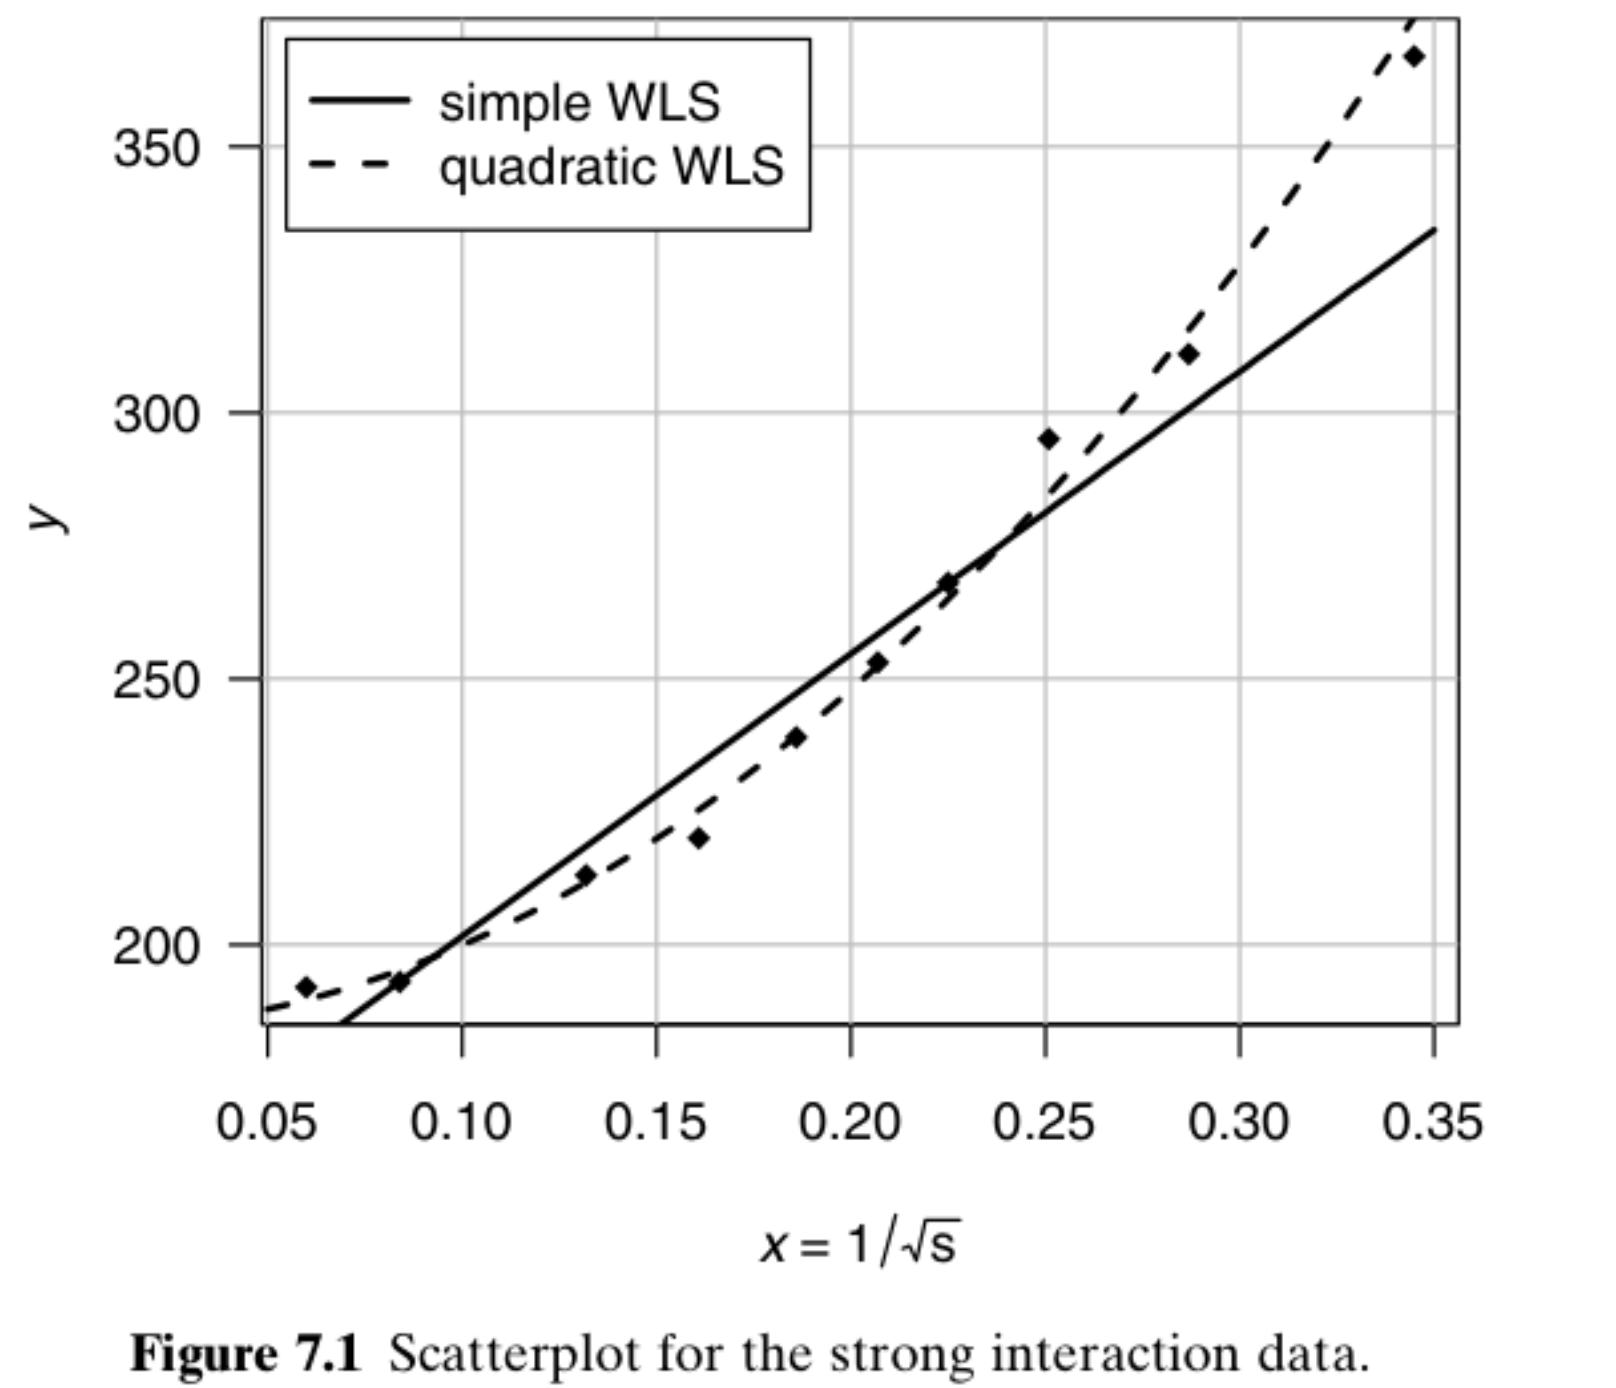
\includegraphics[width=1\textwidth]{fig1.png}
\end{figure}

\section*{Case Study}

\begin{center}
\textbf{\textcolor{teal}{Weighted Least Squares Regression}}

\vspace{1em}
\textbf{\textcolor{teal}{Dose-Response Study for Rosuvastatin in Japanese Patients with High Cholesterol}}

\vspace{2em}
\textcolor{teal}{"Randomized Dose-Response Study of Rosuvastatin in Japanese Patients with Hypercholesterolemia" Saito, et al, Journal of Atherosclerosis, 2003, 10:329-336}
\end{center}
\noindent
\textcolor{teal}{
Errors are independent \\
Variance of errors are not all equal (Heteroscedastic) \\
Variances may be known or estimated \\
Estimates can be obtained by regression when the variance is a power function of the mean \\
General case with known variance structure (up to $\sigma^2$)
}
\[
\text{Var}(e) = \text{Var} \begin{pmatrix} e_1 \\ \vdots \\ e_n \end{pmatrix} = \sigma^2 V = \sigma^2 \begin{pmatrix} v_1 & 0 & \dots & 0 \\ 0 & v_2 & \dots & 0 \\ \vdots & \vdots & \ddots & \vdots \\ 0 & 0 & \dots & v_n \end{pmatrix}
\]
\begin{center}
\textbf{\textcolor{teal}{Weighted Least Squares Procedure}}
\end{center}
\noindent
\textcolor{teal}{
Give higher weights to observations with smaller variances \\
Create a Weight matrix \( W \), that is diagonal with elements equal to reciprocals of square roots of elements of \( V \)
}
\text{Transform the \( Y \) vector and \( X \) matrix by pre-multiplying each by \( W \)}
\[
W = V^{-1/2} = \begin{pmatrix} 1 / \sqrt{v_1} & 0 & \dots & 0 \\ 0 & 1 / \sqrt{v_2} & \dots & 0 \\ \vdots & \vdots & \ddots & \vdots \\ 0 & 0 & \dots & 1 / \sqrt{v_n} \end{pmatrix}
\]
\[
X^* = W X \quad \text{and} \quad Y^* = W Y \quad \Rightarrow \quad \hat{\beta}_W = (X^{*'} X^*)^{-1} X^{*'} Y^*
\]
\textbf{\textcolor{teal}{Example – Cholesterol Drug Dose-Response Study}}\\
- \textcolor{teal}{Study of Drug Rosuvastatin in Japanese Patients with high cholesterol}\\
- \textcolor{teal}{6 Doses – 1, 2.5, 5, 10, 20, 40}\\
- \textcolor{teal}{Response - \% Change in LDL Cholesterol @ week 12}\\
- \textcolor{teal}{Data Reported – Group Means by Dose}\\
- \textcolor{teal}{Sample sizes Varied by dose}\\
- \textcolor{teal}{Assuming equal variance among individual patients:}\\
$\quad \textcolor{teal}{V\left(\bar{Y}_j\right) = \frac{\sigma^2}{n_j}} \quad j = 1, \ldots, 6$

\textbf{\textcolor{teal}{Data and \( Y, Y^*, X, X^*, V \) and \( W \)}}
\begin{figure}[H]
    \centering
    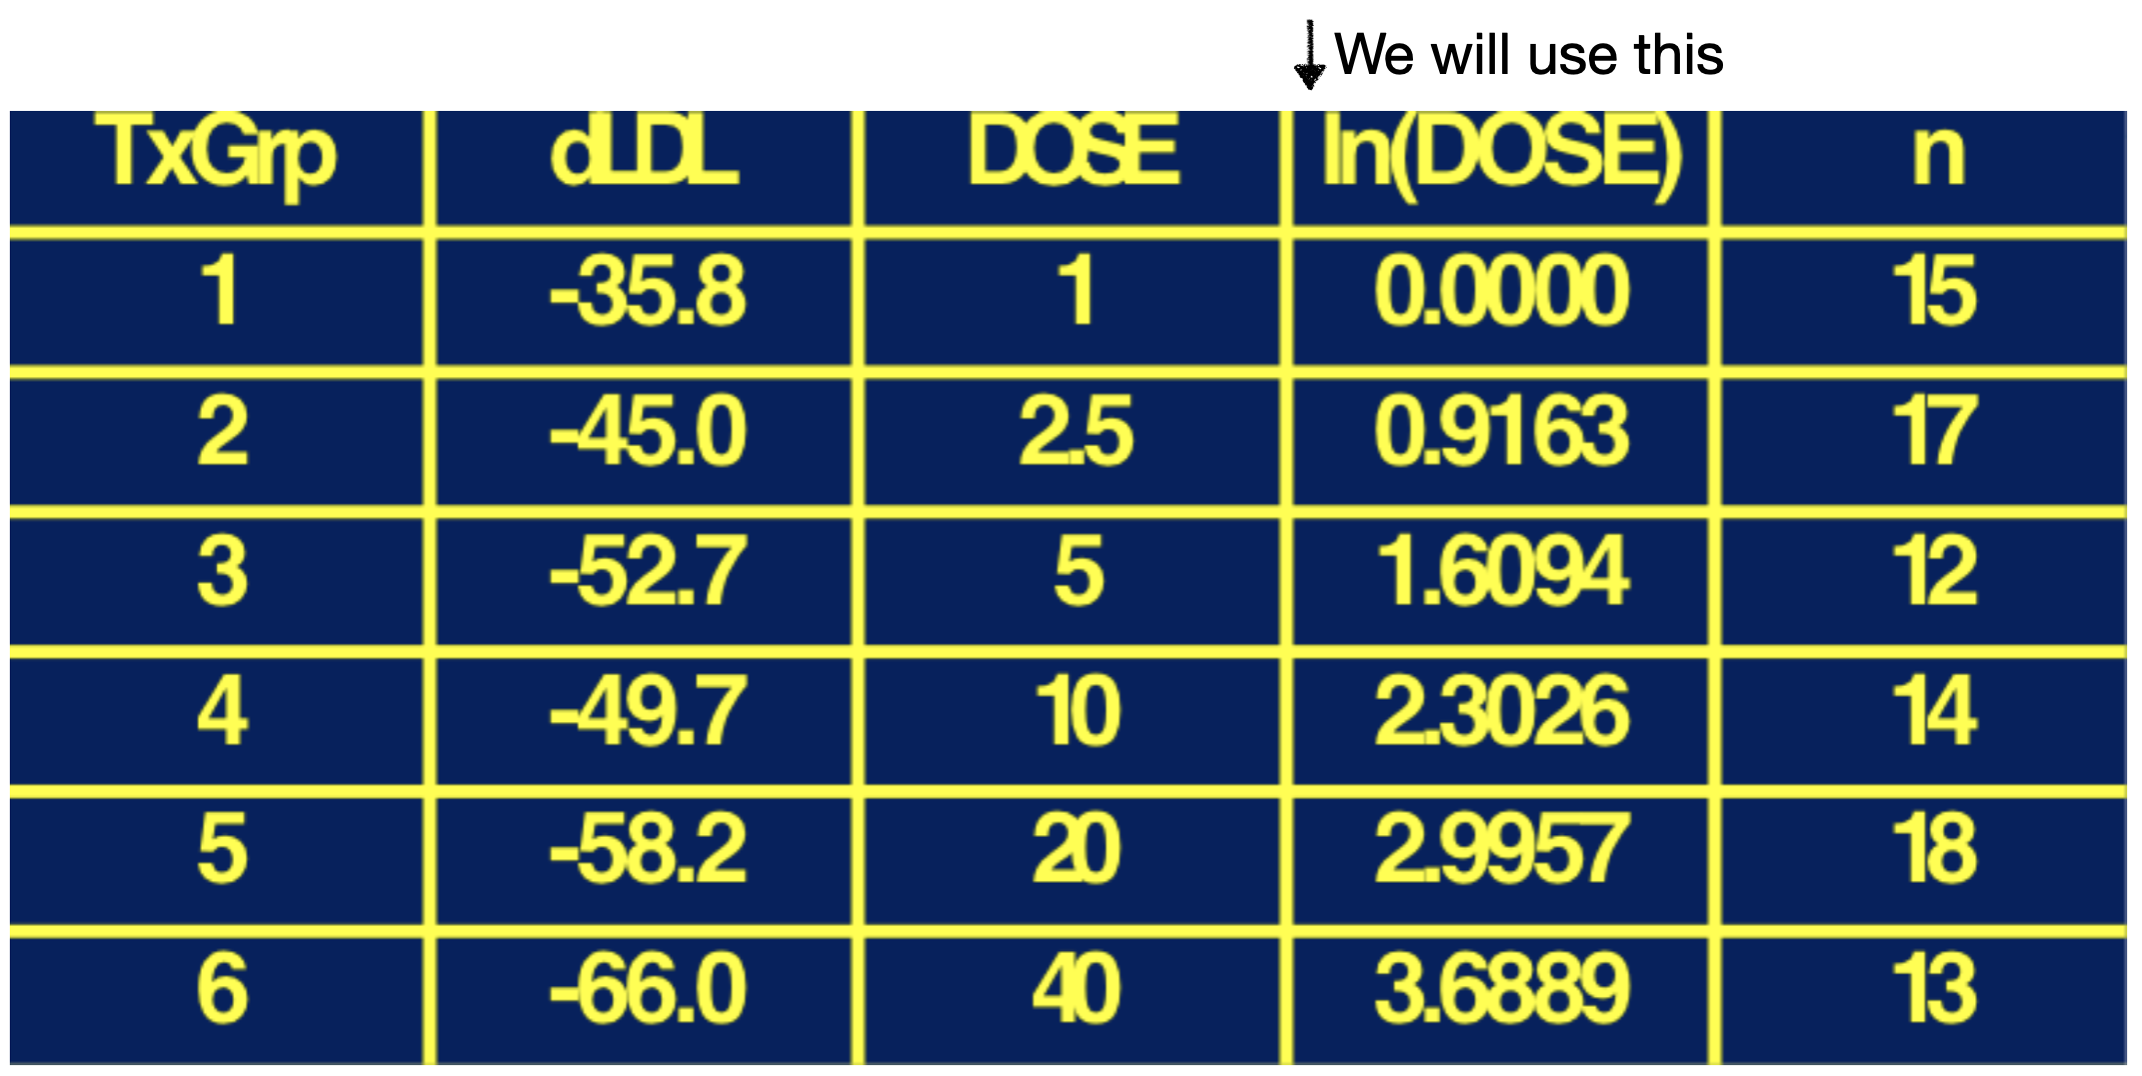
\includegraphics[width=0.55\textwidth]{fig2.png}
\end{figure}     
\begin{figure}[H]
    \centering
    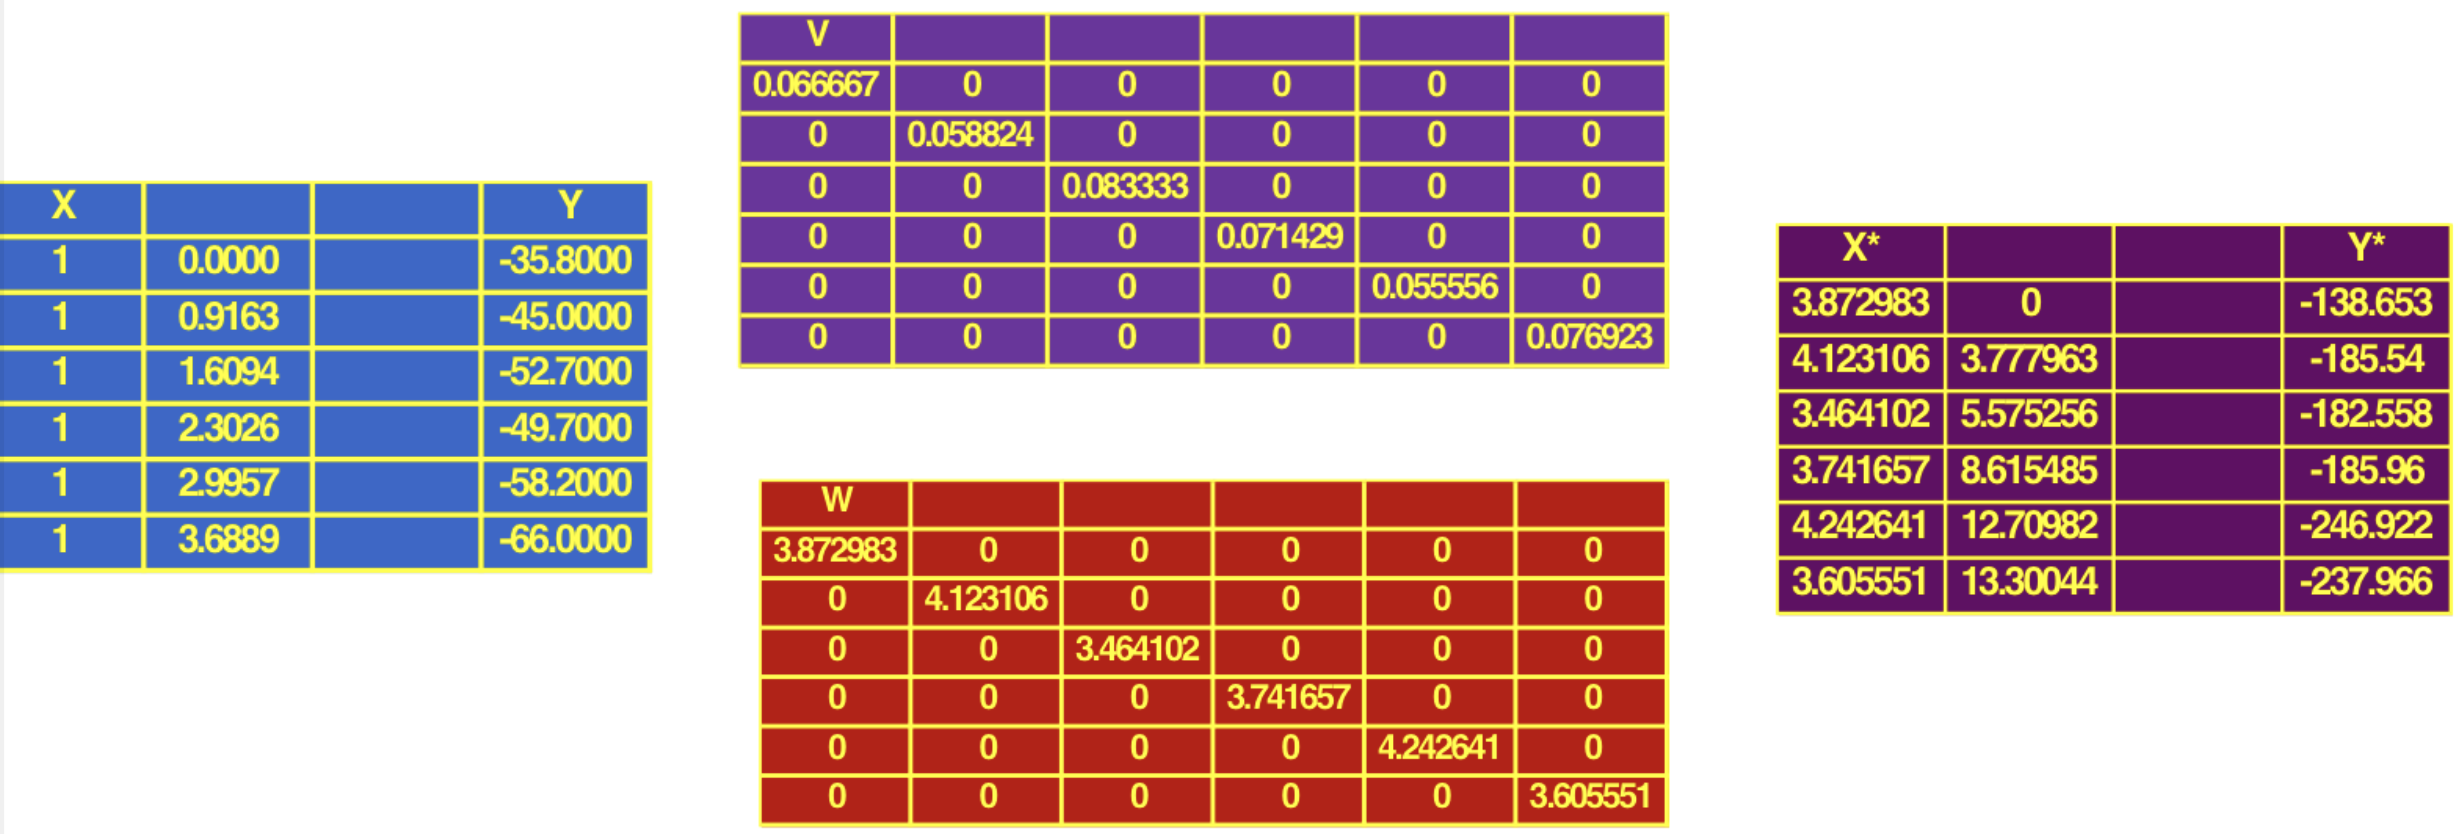
\includegraphics[width=1\textwidth]{fig3.png}
\end{figure}     
\begin{figure}[H]
    \centering
    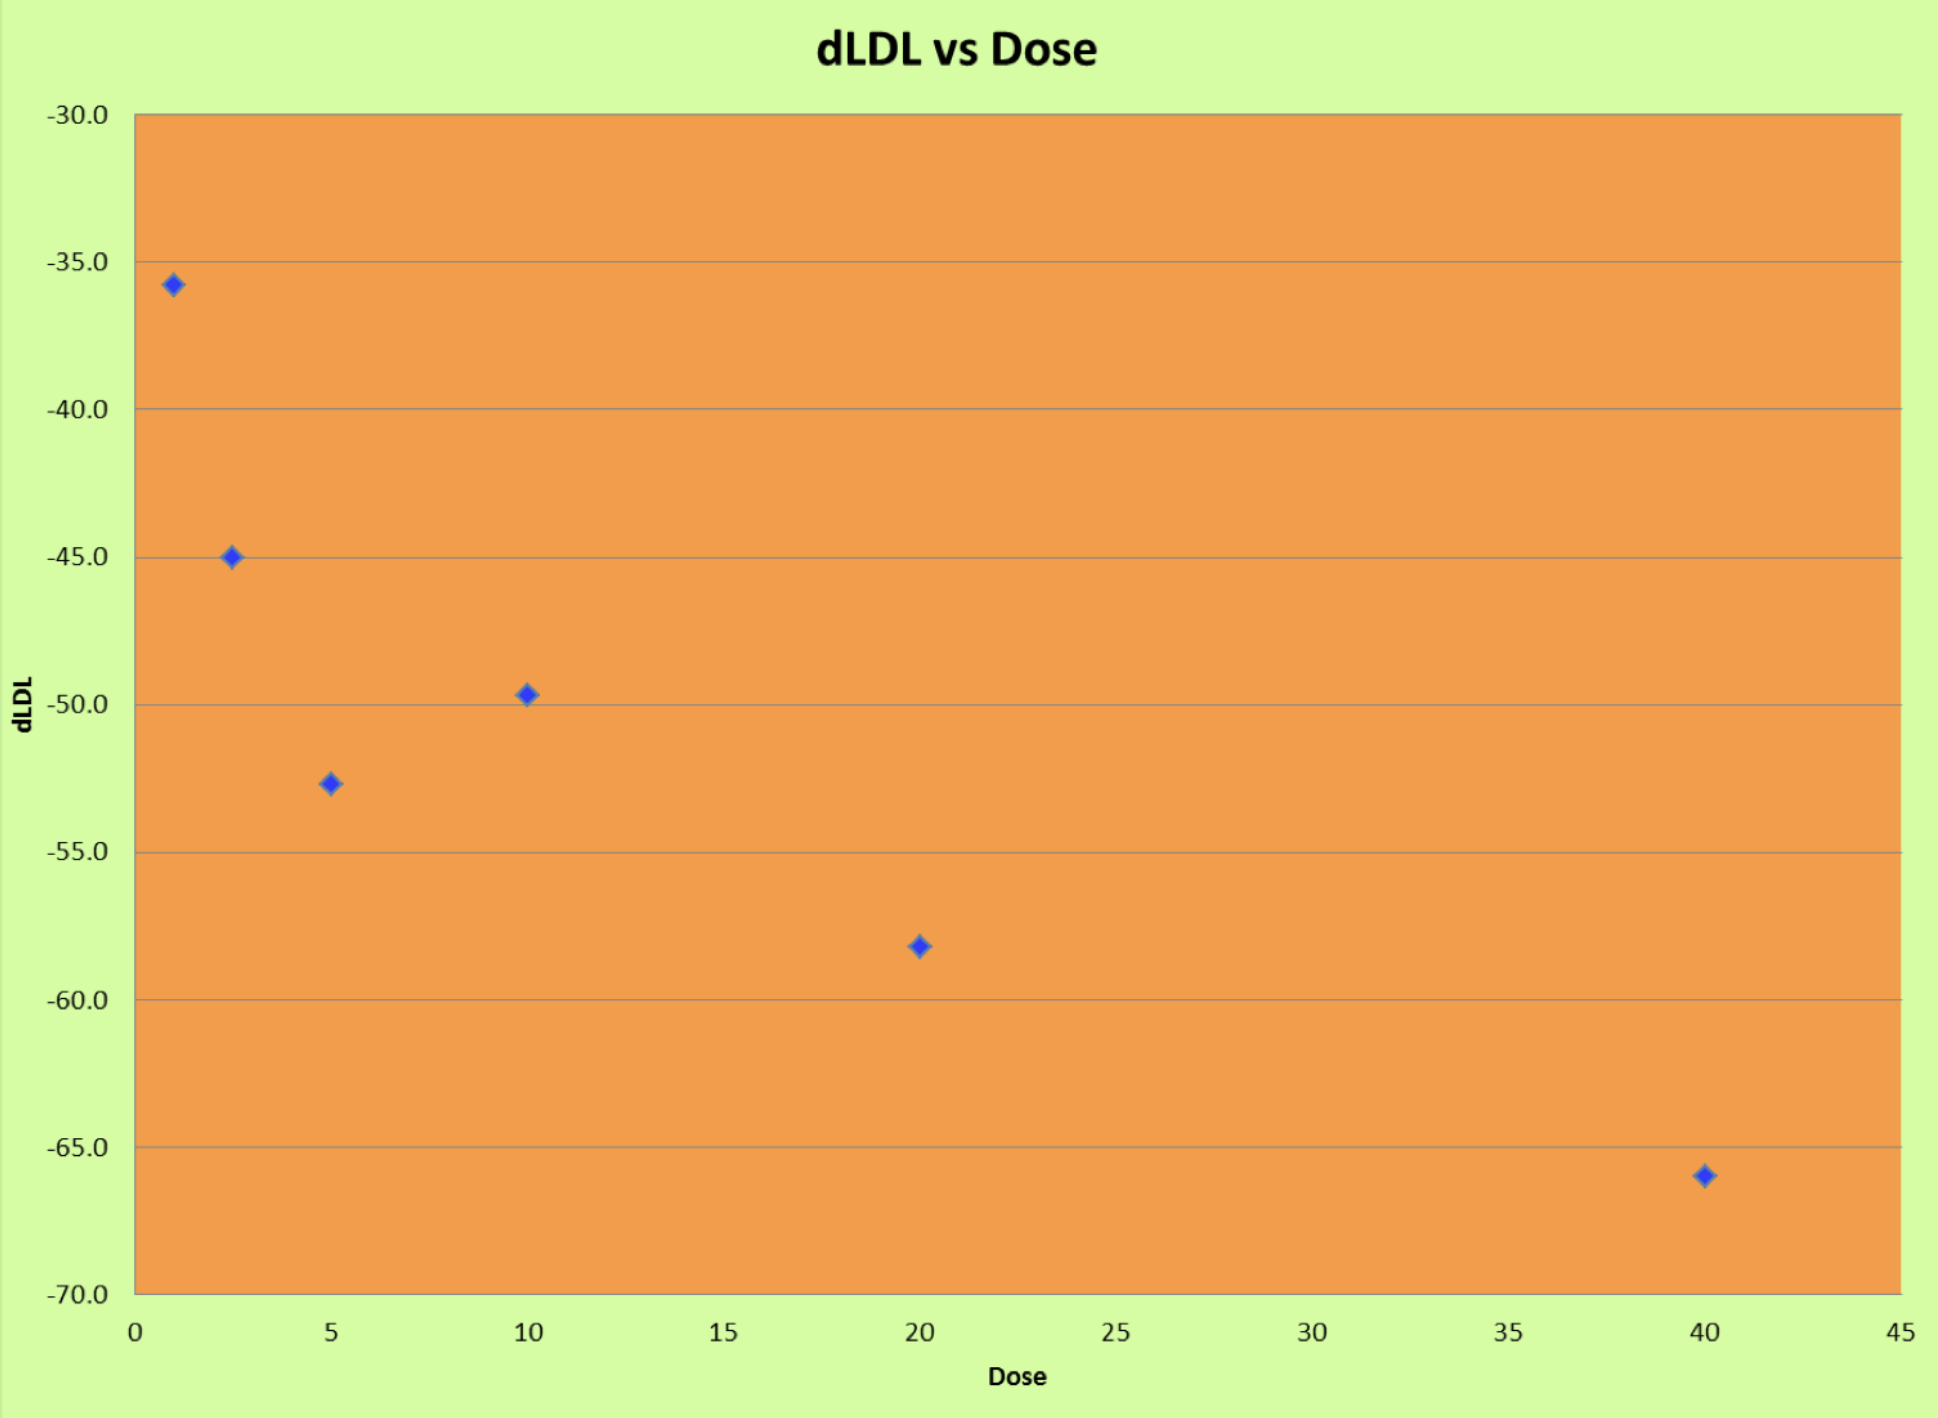
\includegraphics[width=0.9\textwidth]{fig4.png}
\end{figure}   
\begin{figure}[H]
    \centering
    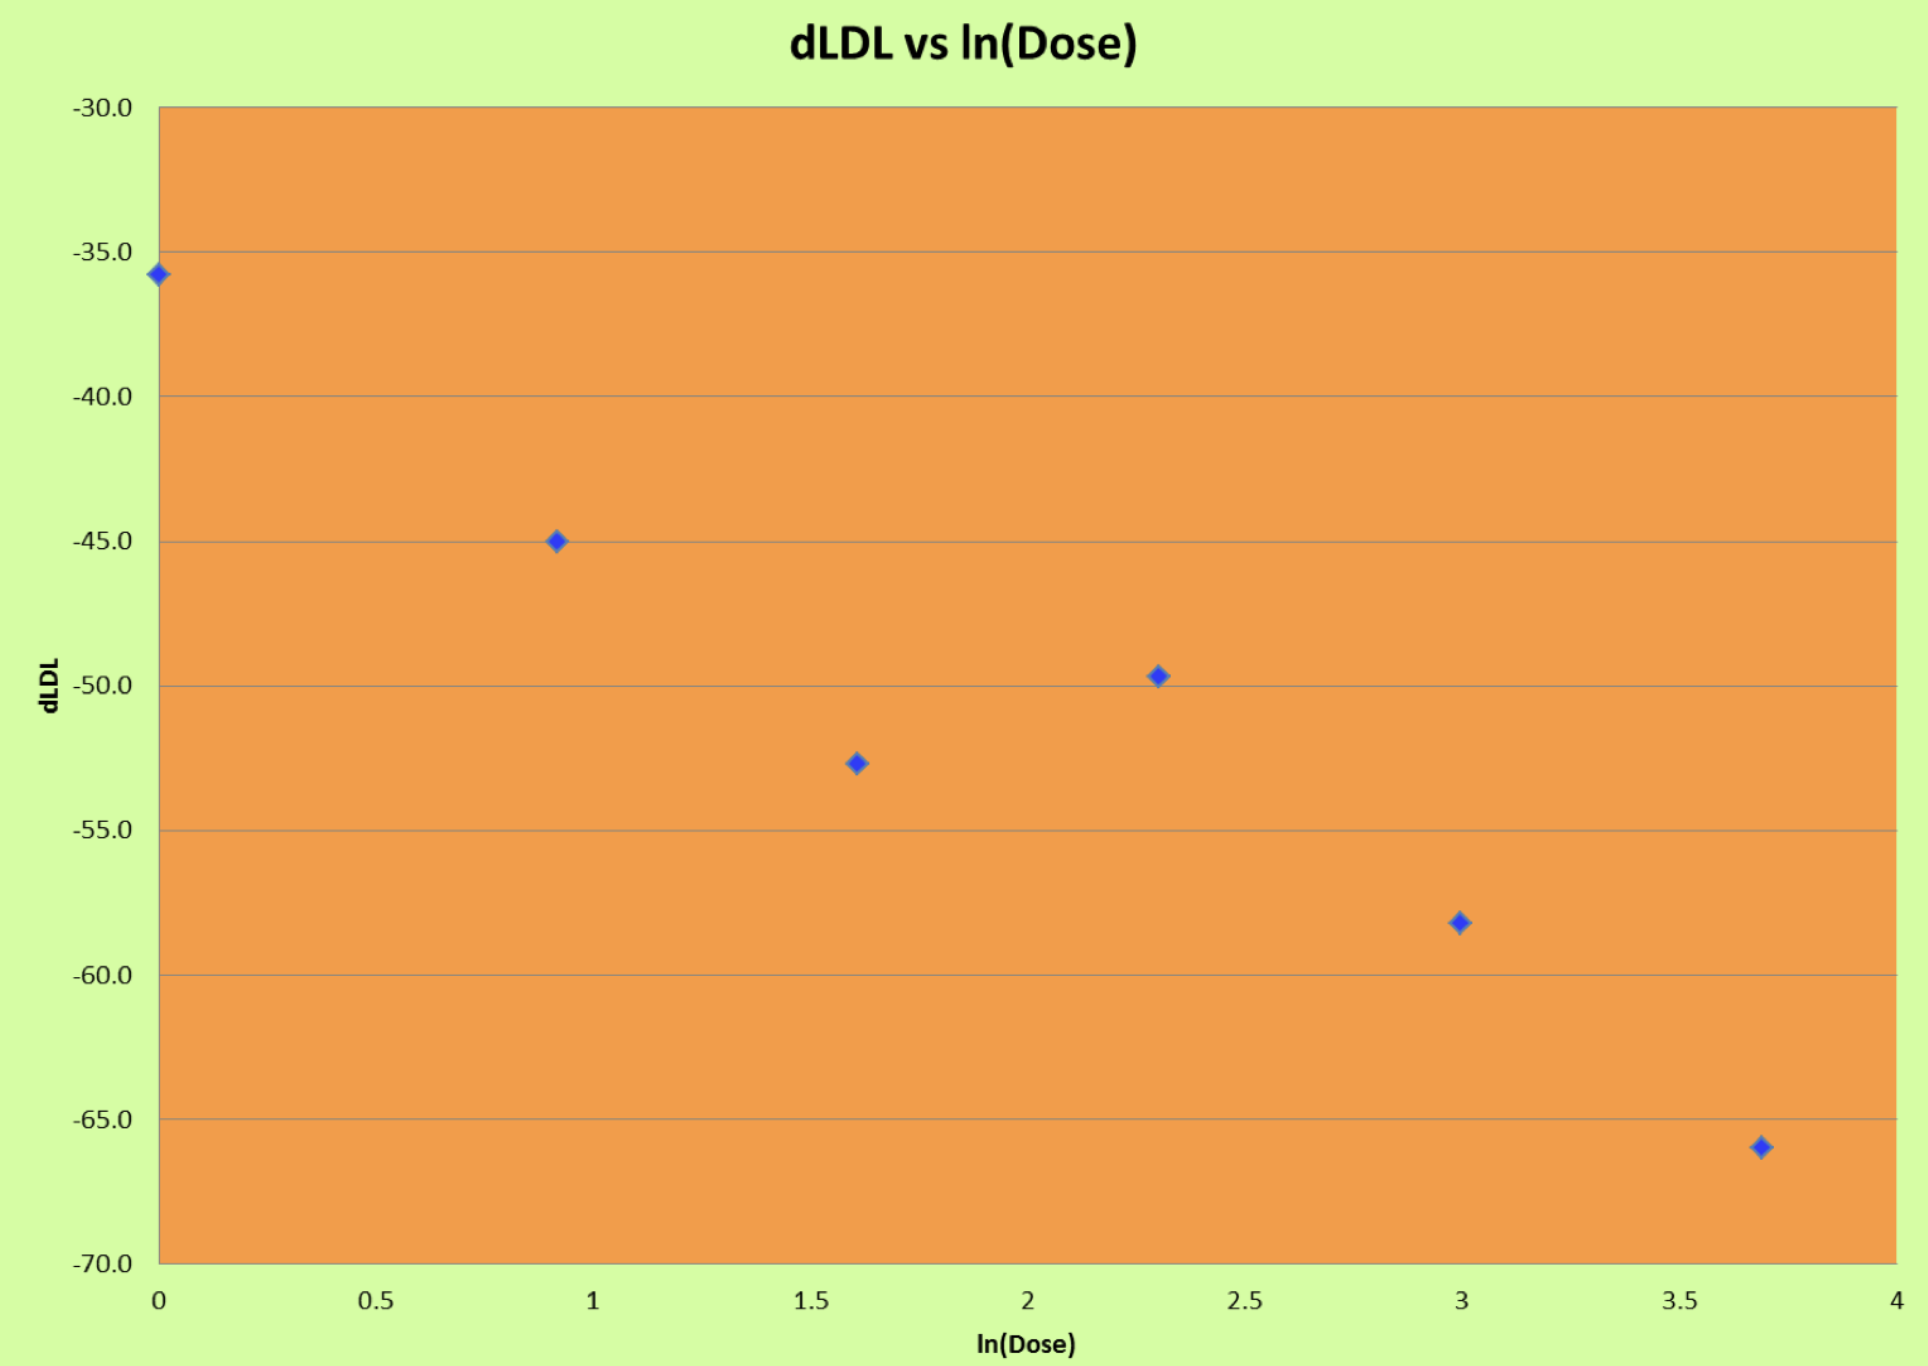
\includegraphics[width=0.9\textwidth]{fig5.png}
\end{figure}   
\textbf{\textcolor{teal}{WLS Regression Estimates, Fitted Values, Residuals}}
\begin{figure}[H]
    \centering
    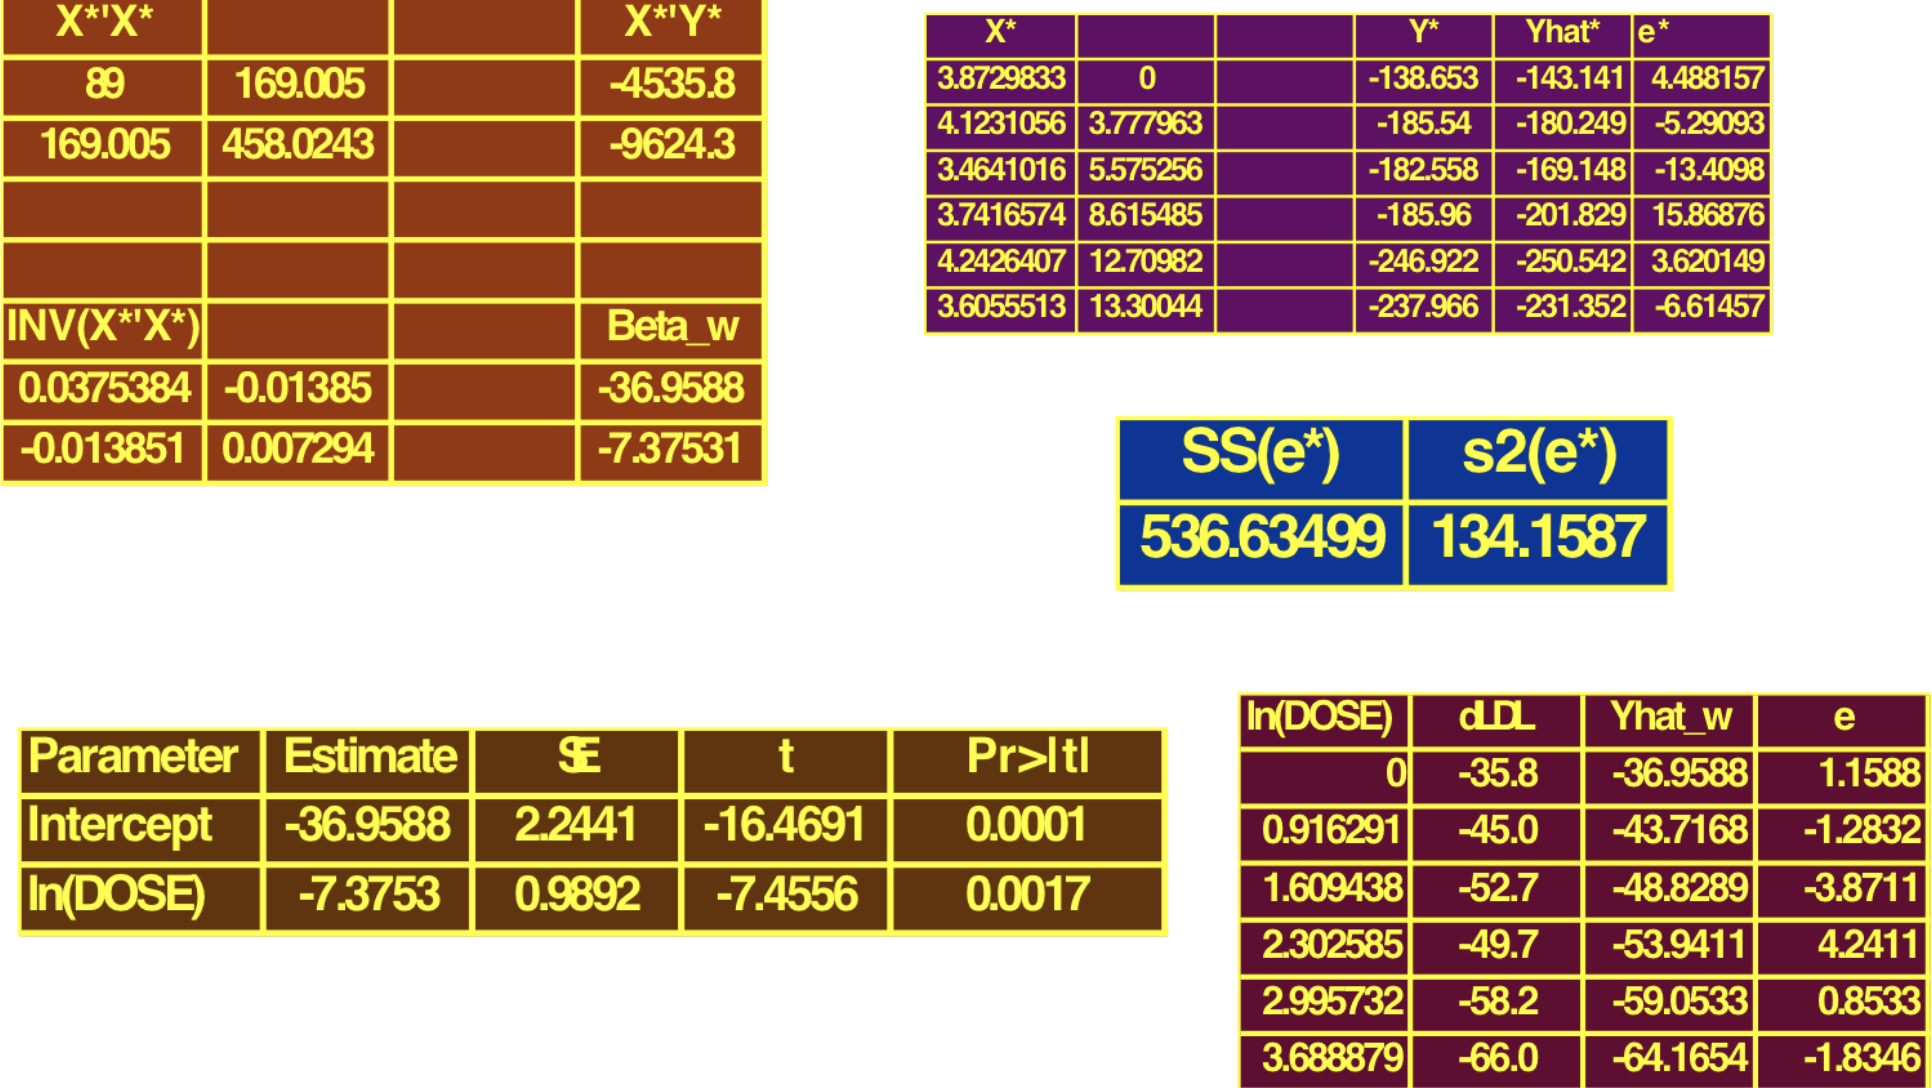
\includegraphics[width=1\textwidth]{fig6.png}
\end{figure}   
\begin{figure}[H]
    \centering
    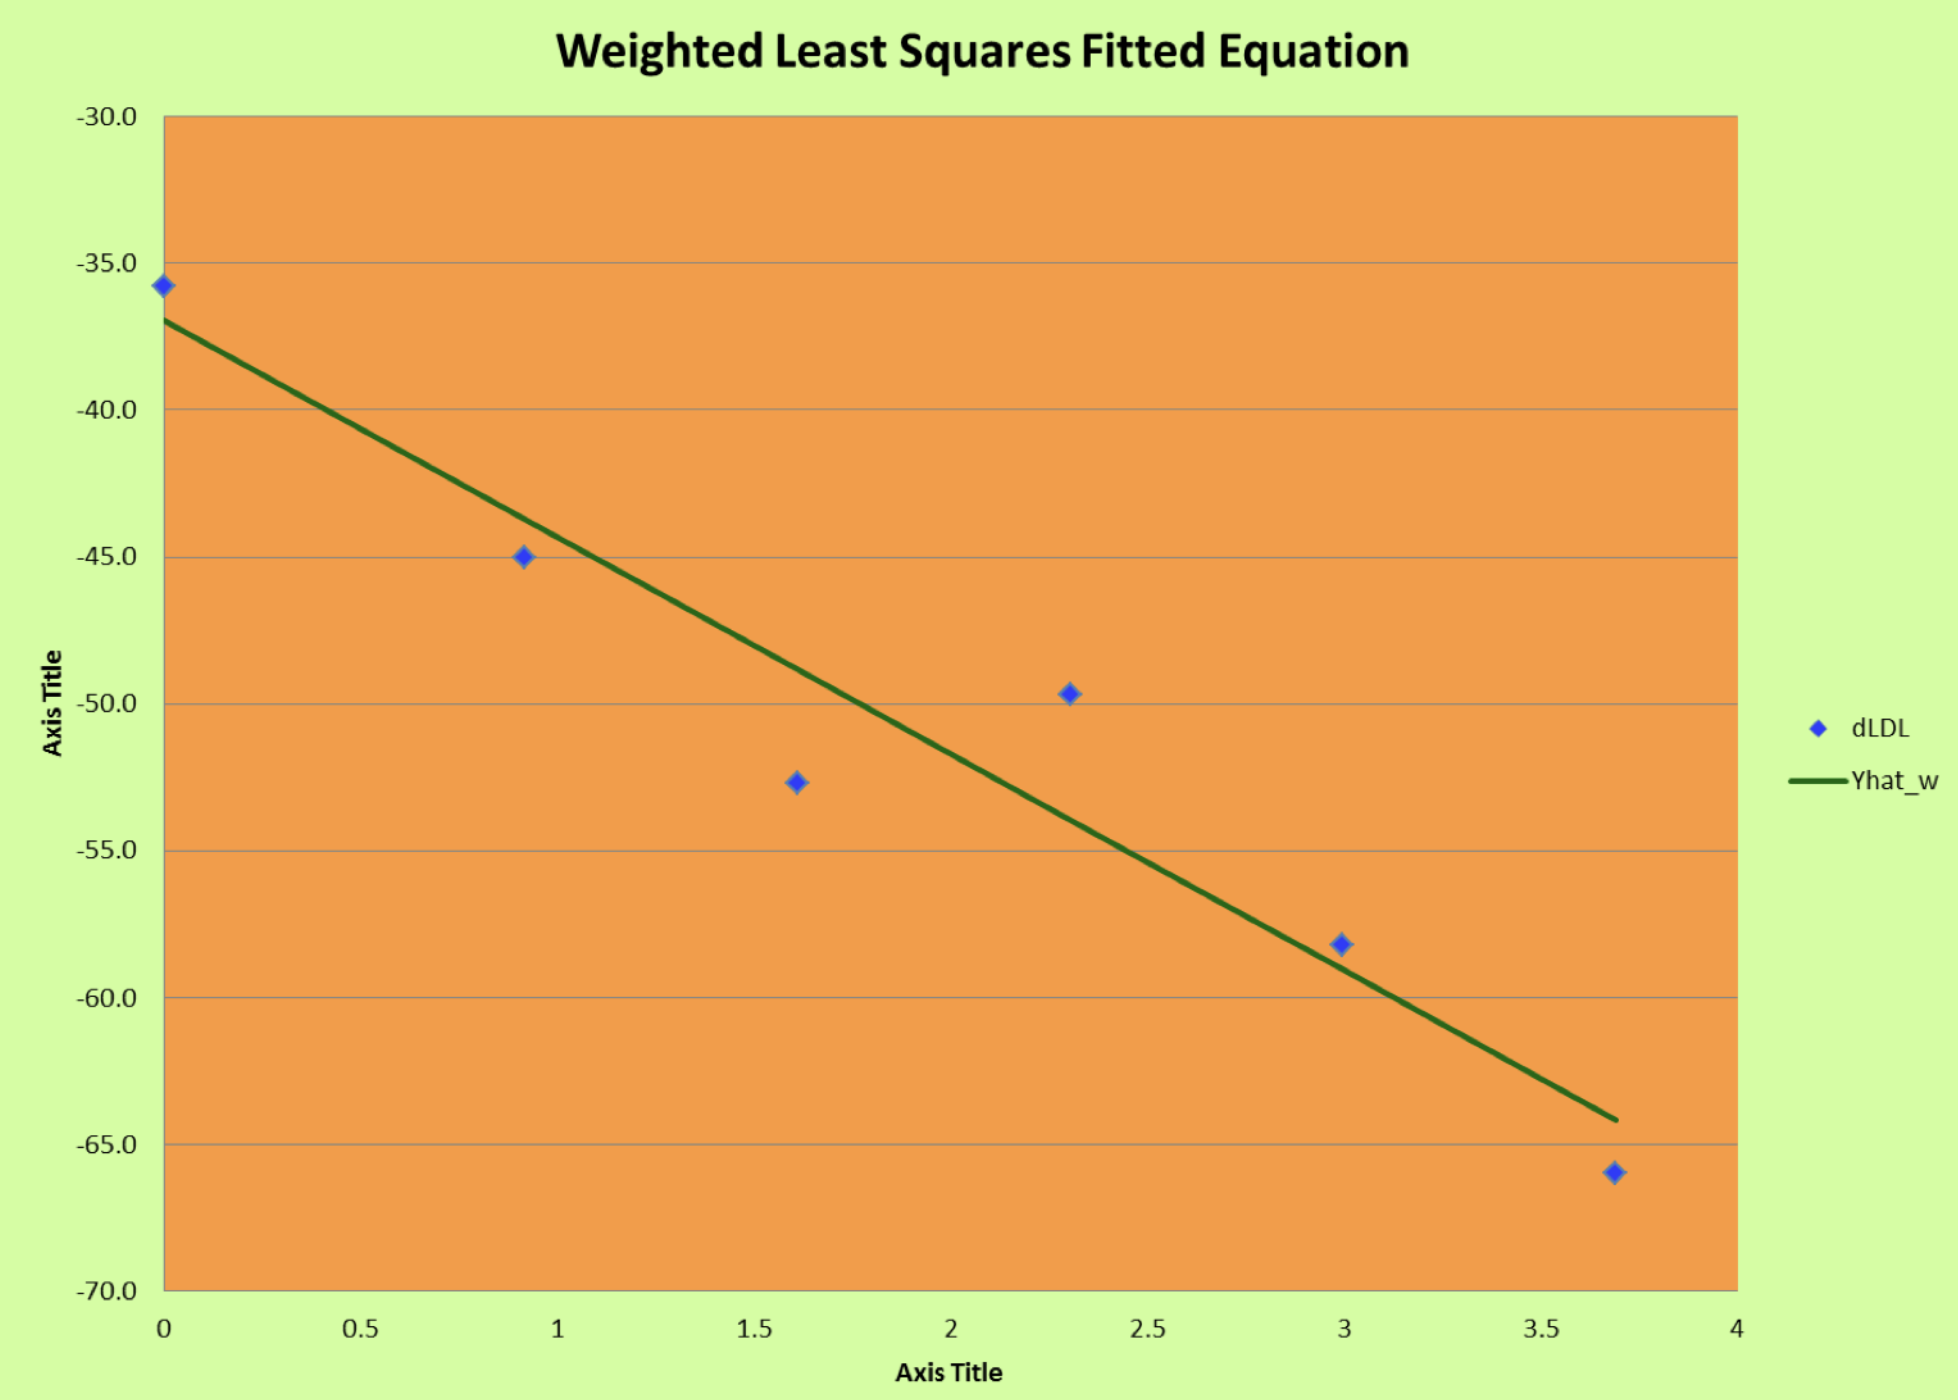
\includegraphics[width=1\textwidth]{fig7.png}
\end{figure}   
\section*{Misspecified Variances}

Suppose the true regression model is
\[
E(Y | X) = X \beta, \quad \text{Var}(Y | X) = \sigma^2 W^{-1},
\]
\noindent
where \( W \) has positive weights on the diagonal and zeros elsewhere. We get the weights wrong, and fit the model using OLS with the estimator
\[
\hat{\beta}^{\text{OLS}} = (X'X)^{-1} X'Y.
\]
\text{Similar to the correct WLS estimate,}
\[
E(\hat{\beta}^{\text{OLS}} | X) = \beta
\]
However,
\[
\text{Var}(\hat{\beta}^{\text{OLS}} | X) = \sigma^2 (X'X)^{-1} (X'W^{-1}X) (X'X)^{-1}
\]
\quad \quad \quad \quad \quad \quad \quad \quad \quad \quad \quad \quad \quad \quad \quad \quad \quad \textcolor{green}{\text{"Sandwich" form}}
\[
\textcolor{red}{\Rightarrow \text{Confidence statements and tests can be incorrect.}}
\]
\section*{Accommodating Incorrect Variances}
\noindent
To estimate \( \text{Var}(\hat{\beta}^{\text{OLS}} | X) \) requires estimating \( \sigma^2 W^{-1} \).\\
Let \( \hat{e}_i = y_i - \hat{\beta'}^{\text{OLS}}x_i \) \textcolor{red}{\text{(i-th residual from misspecified model)}}.\\
Can estimate \( \sigma^2 / w_i \) by \( \hat{e}_i^2 \).\\
If we replace \( \sigma^2 W^{-1} \) by a diagonal matrix with \( \hat{e}_i^2 \) on the diagonal, this produces a consistent estimate of \( \text{Var}(\hat{\beta}^{\text{OLS}} | X) \).\\
An alternative version of this is called the \textcolor{blue}{sandwich} estimator.\\
$\text{Var}(\hat{\beta}^{\text{OLS}} | X) = (X'X)^{-1} [X' \, \text{diag} \left( \frac{\hat{e}_i^2}{(1 - h_{ii})^2} \right) X] (X'X)^{-1}$\\
\textcolor{red}{\text{i-th leverage (to be discussed soon).}}

\noindent
\textbf{Sniffer Data}\\
When gasoline is pumped into a tank, hydrocarbon vapors are forced out of the tank and into the atmosphere. To reduce this significant source of air pollution, devices are installed to capture the vapor. In testing these vapor recovery systems, a “sniffer” measures the amount recovered. To estimate the efficiency of the system, some method of estimating the total amount given off must be used. To this end, a laboratory experiment was conducted in which the amount of vapor given off was measured under controlled conditions. Four predictors are relevant for modeling:
\[
\textcolor{red}{\text{Predictors: }}
\begin{aligned}
    &\text{TankTemp} = \text{initial tank temperature (degrees F)} \\
    &\text{GasTemp} = \text{temperature of the dispensed gasoline (degrees F)} \\
    &\text{TankPres} = \text{initial vapor pressure in the tank (psi)} \\
    &\text{GasPres} = \text{vapor pressure of the dispensed gasoline (psi)}
\end{aligned}
\]
\textbf{Response:} \text{the hydrocarbons \( Y \) emitted in grams.}
\begin{figure}[H]
    \centering
    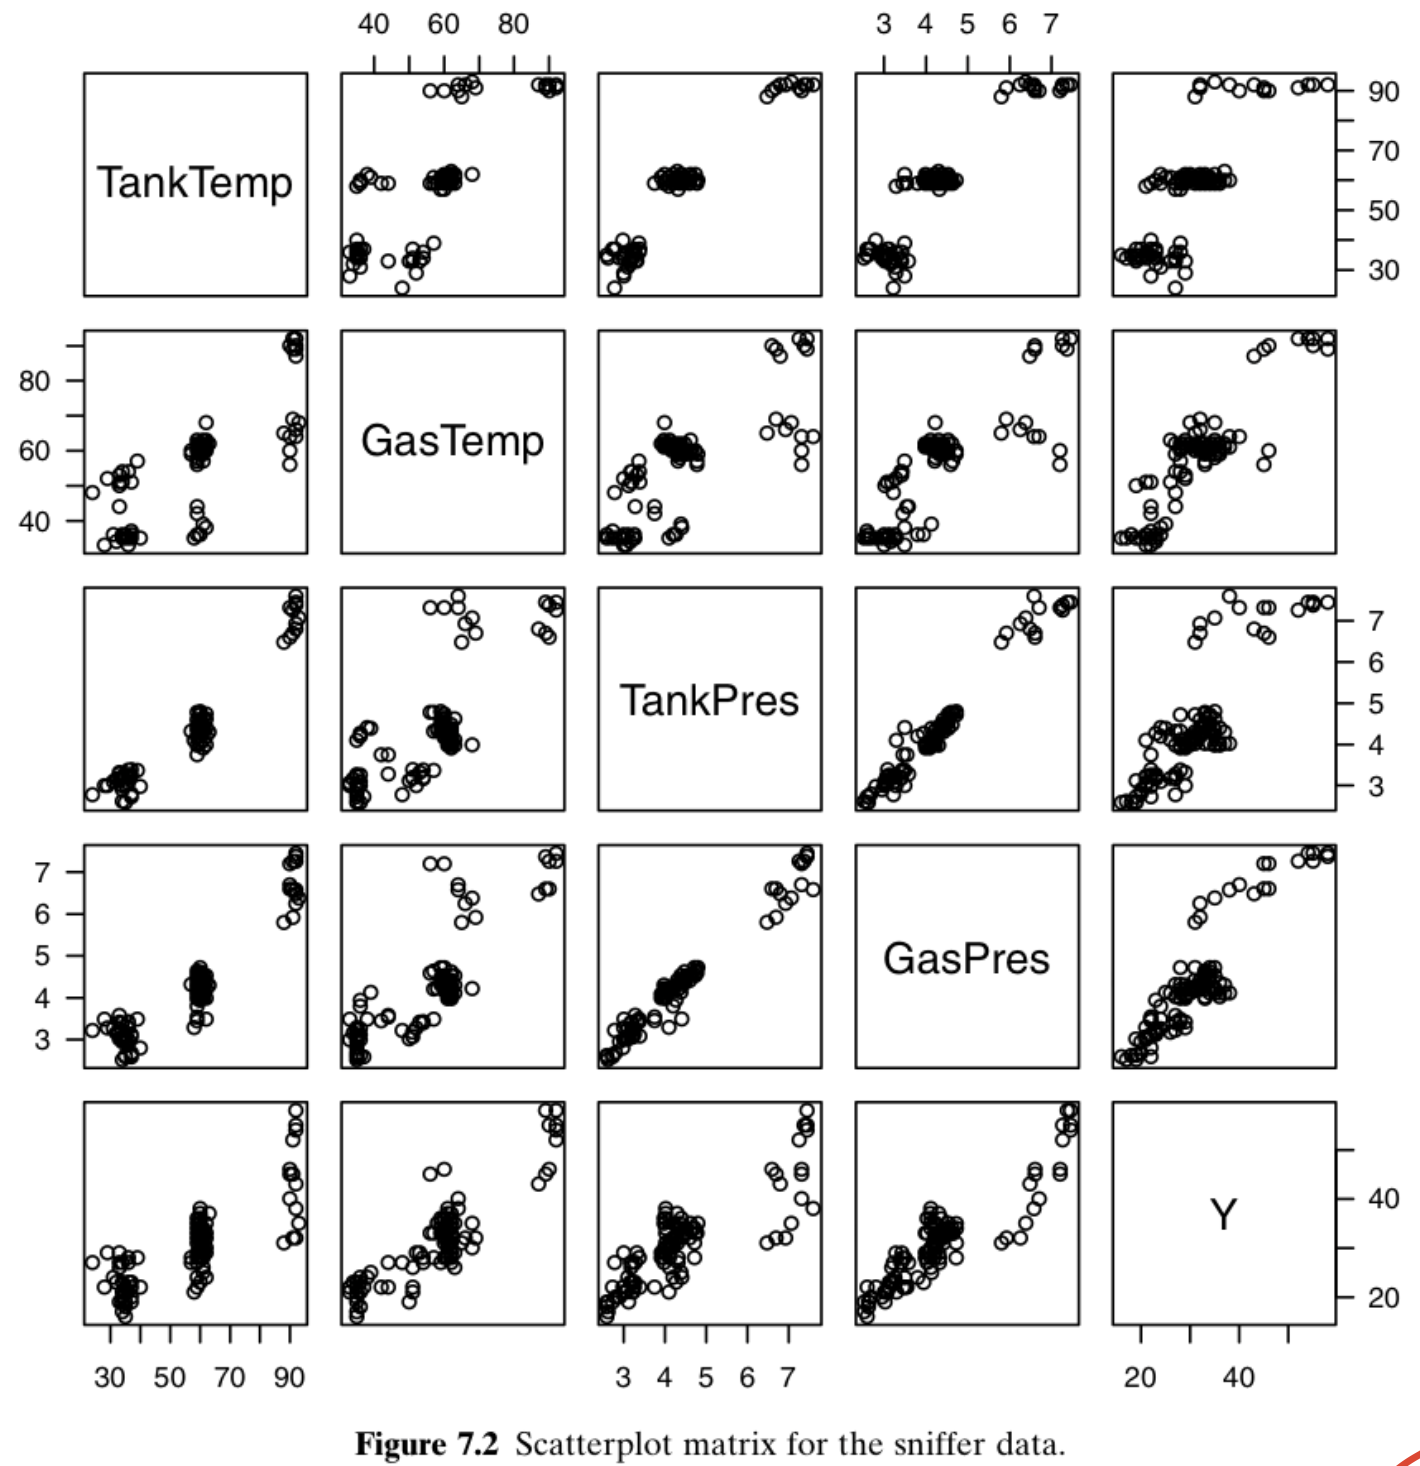
\includegraphics[width=1\textwidth]{fig8.png}
\end{figure} 
\begin{figure}[H]
    \centering
    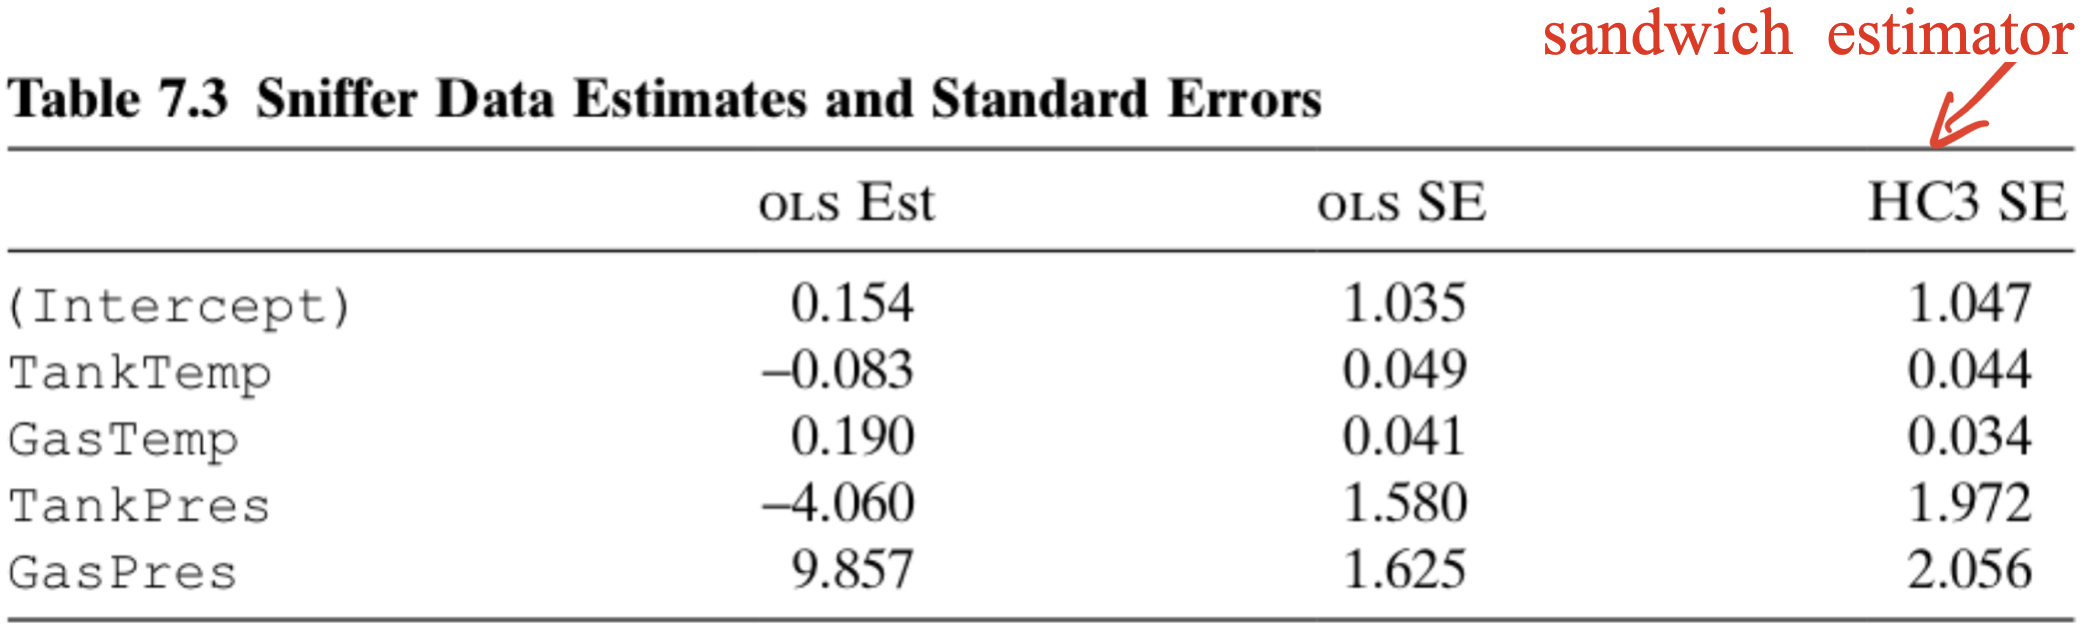
\includegraphics[width=1\textwidth]{fig9.png}
\end{figure} 

\subsection*{A Test for Constant Variance}

\noindent
Suppose that for some parameter vector \( \lambda \) and some vector of regressors \( Z \)
\[
\text{Var}(Y | X, Z = z) = \sigma^2 \exp(\lambda' z),
\]
where \( w = \exp(-\lambda' z) \).\\
If \( \lambda = 0 \Rightarrow \text{constant variance} \)\\
Therefore to test\\
$H_0: \lambda = 0$\\
$H_1: \lambda \neq 0$\\
is a test for nonconstant variance.\\
Great latitude in specifying \( Z \).\\
\textit{e.g., if \( Z = Y \), then variance depends on response.}\\
\textit{e.g., \( Z \) could be same as \( X \) or a subset of \( X \).}\\
With normal errors assumed, can derive a \textcolor{blue}{score} test that has approximate \( \chi^2(g) \) under \( H_0 \).
\textcolor{red}{g = \# \text{ regressors in } Z}\\
$\Rightarrow \text{p-value}$
\begin{figure}[H]
    \centering
    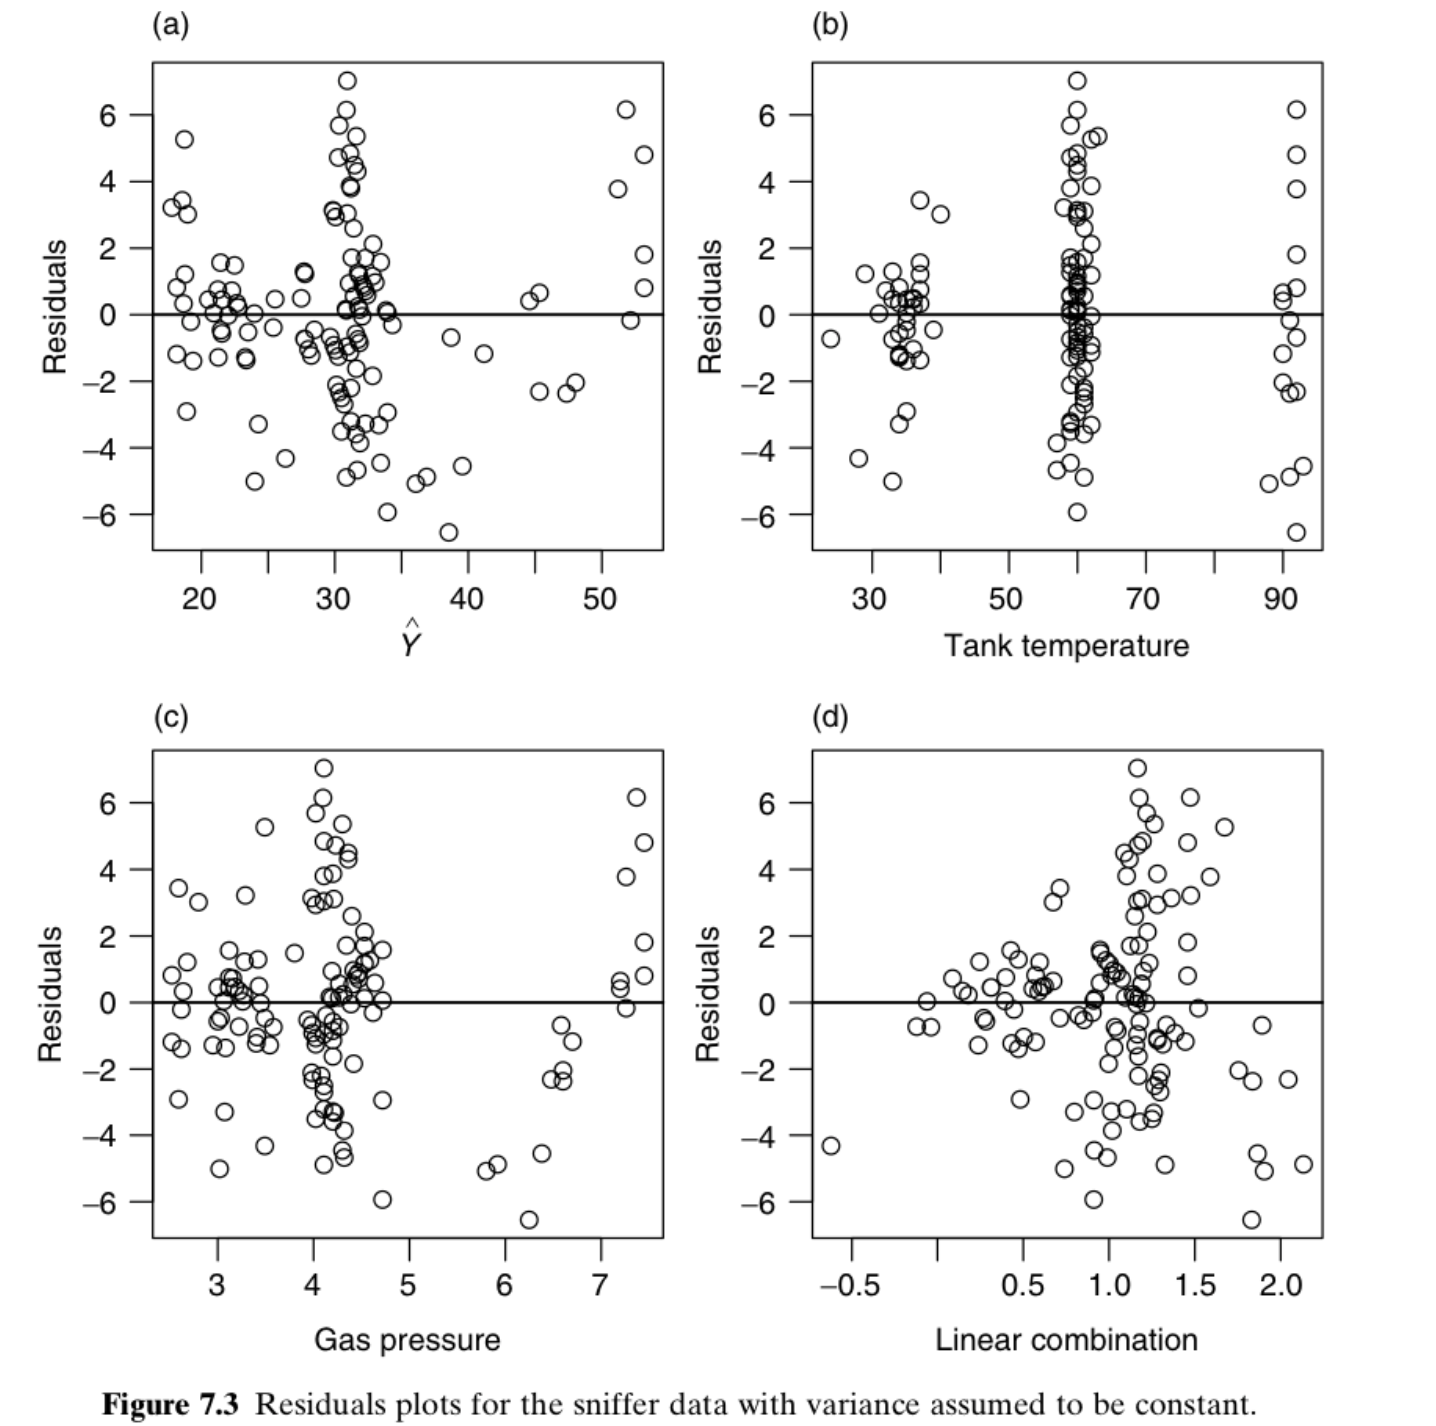
\includegraphics[width=1\textwidth]{fig10.png}
\end{figure} 
\begin{figure}[H]
    \centering
    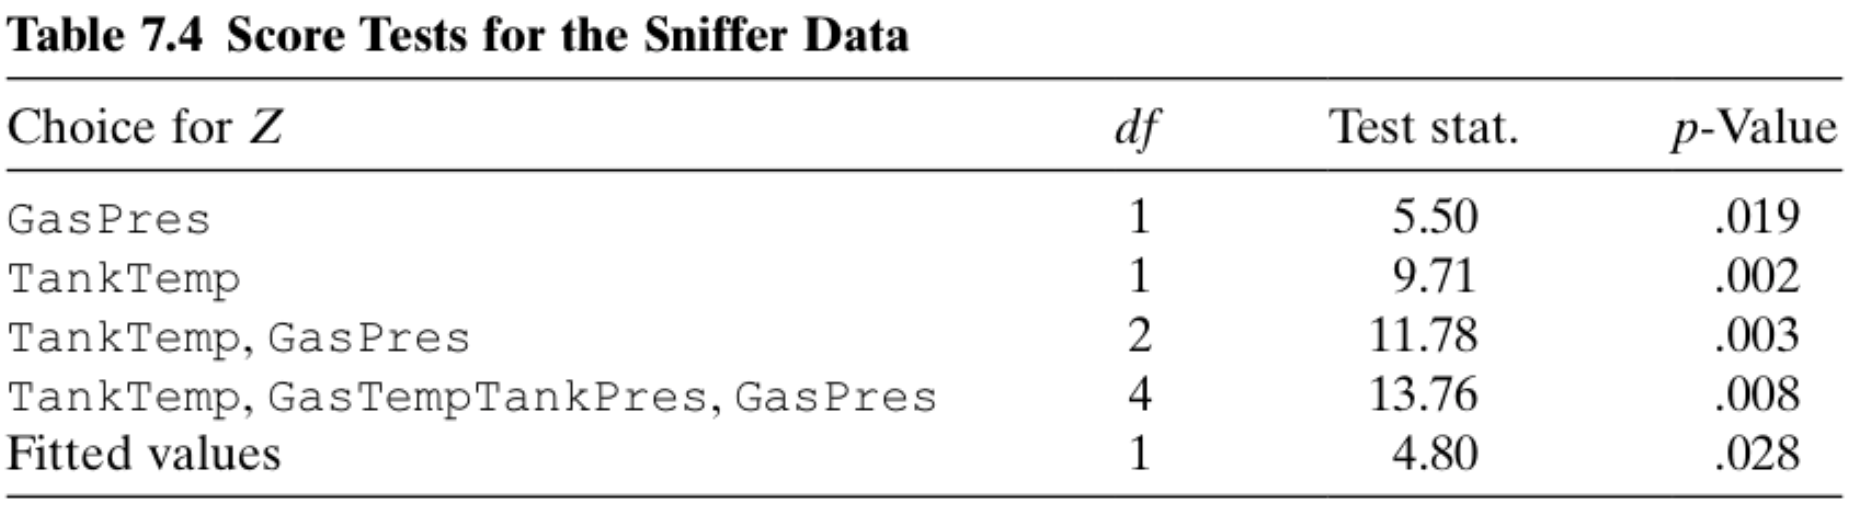
\includegraphics[width=1\textwidth]{fig11.png}
\end{figure} 

\section*{General Correlation Structures}
\noindent
The generalized least squares or GLS model extends WLS one step further, and starts with
\[
E(Y | X) = X \beta, \quad \text{Var}(Y | X) = \Sigma,
\]
where \( \Sigma \) is an \( n \times n \) positive definite symmetric matrix. The WLS model uses \( \Sigma = \sigma^2 W^{-1} \) for a diagonal matrix \( W \), and the OLS model uses \( \Sigma = \sigma^2 I \).
If we have \( n \) observations and \( \Sigma \) is completely unknown, then \( \Sigma \) contains \( n(n - 1)/2 \) parameters, which is much larger than the number of observations \( n \). The only hope is to introduce some structure in \( \Sigma \). Here are some examples.\\
\textbf{Compound Symmetry}\\
If all the observations are equally correlated, then
\[
\Sigma_{CS} = \sigma^2 \begin{pmatrix} 
1 & \rho & \cdots & \rho \\
\rho & 1 & \cdots & \rho \\
\vdots & \vdots & \ddots & \vdots \\
\rho & \rho & \cdots & 1 
\end{pmatrix},
\]
\noindent
which has only two parameters \( \rho \) and \( \sigma^2 \). Generalized least squares software, such as the \texttt{gls} function in the \texttt{nlme} package, can be used for estimation.\\
\textbf{Autoregressive} \\
This form is generally associated with time series. If data are time ordered and equally spaced, the lag-1 autoregressive covariance structure is
\[
\Sigma_{AR} = \sigma^2 \begin{pmatrix} 
1 & \rho & \cdots & \rho^{n-1} \\
\rho & 1 & \cdots & \rho^{n-2} \\
\vdots & \vdots & \ddots & \vdots \\
\rho^{n-1} & \rho^{n-2} & \cdots & 1 
\end{pmatrix},
\]
which also contains only two parameters.\\
\textbf{Block Diagonal} \\
A block diagonal form for \( \Sigma \) can arise if observations are sampled clusters. For example, a study of school performance might sample \( m \) children from each of \( k \) classrooms. The \( m \) children within a classroom may be correlated because they all have the same teacher, but children in different classrooms are independent.
\section*{Random Coefficient Models}
\noindent
The random coefficient model, as a special case of mixed models, allows for appropriate inferences. Consider a population regression mean function
\[
E(y | \text{loudness} = x) = \beta_0 + \beta_1 x,
\]
where subject effects are not allowed. To add them, we hypothesize that each of the subjects may have his or her own slope and intercept. Let \( y_{ij}, i = 1, \ldots, 10, j = 1, \ldots, 5 \) be the log-response for subject \( i \) measured at the \( j \)th level of loudness.
For the \( i \)th subject,
\[
E(y_{ij} | \text{loudness} = x, b_{0i}, b_{1i}) = (\beta_0 + b_{0i}) + (\beta_1 + b_{1i}) \, \text{loudness}_{ij},
\]
where \( b_{0i} \) and \( b_{1i} \) are the deviations from the population intercept and slope for the \( i \)th subject, and they are treated as random variables,
\[
\begin{pmatrix} b_{0i} \\ b_{1i} \end{pmatrix} \sim N \left( \begin{pmatrix} 0 \\ 0 \end{pmatrix}, \begin{pmatrix} \tau_0^2 & \tau_{01} \\ \tau_{01} & \tau_1^2 \end{pmatrix} \right).
\]
Inferences about \( (\beta_0, \beta_1) \) concern population behavior. Inferences about \( (\tau_0^2, \tau_1^2) \) concern the variation of the intercepts and slopes between individuals in the population.
\begin{figure}[H]
    \centering
    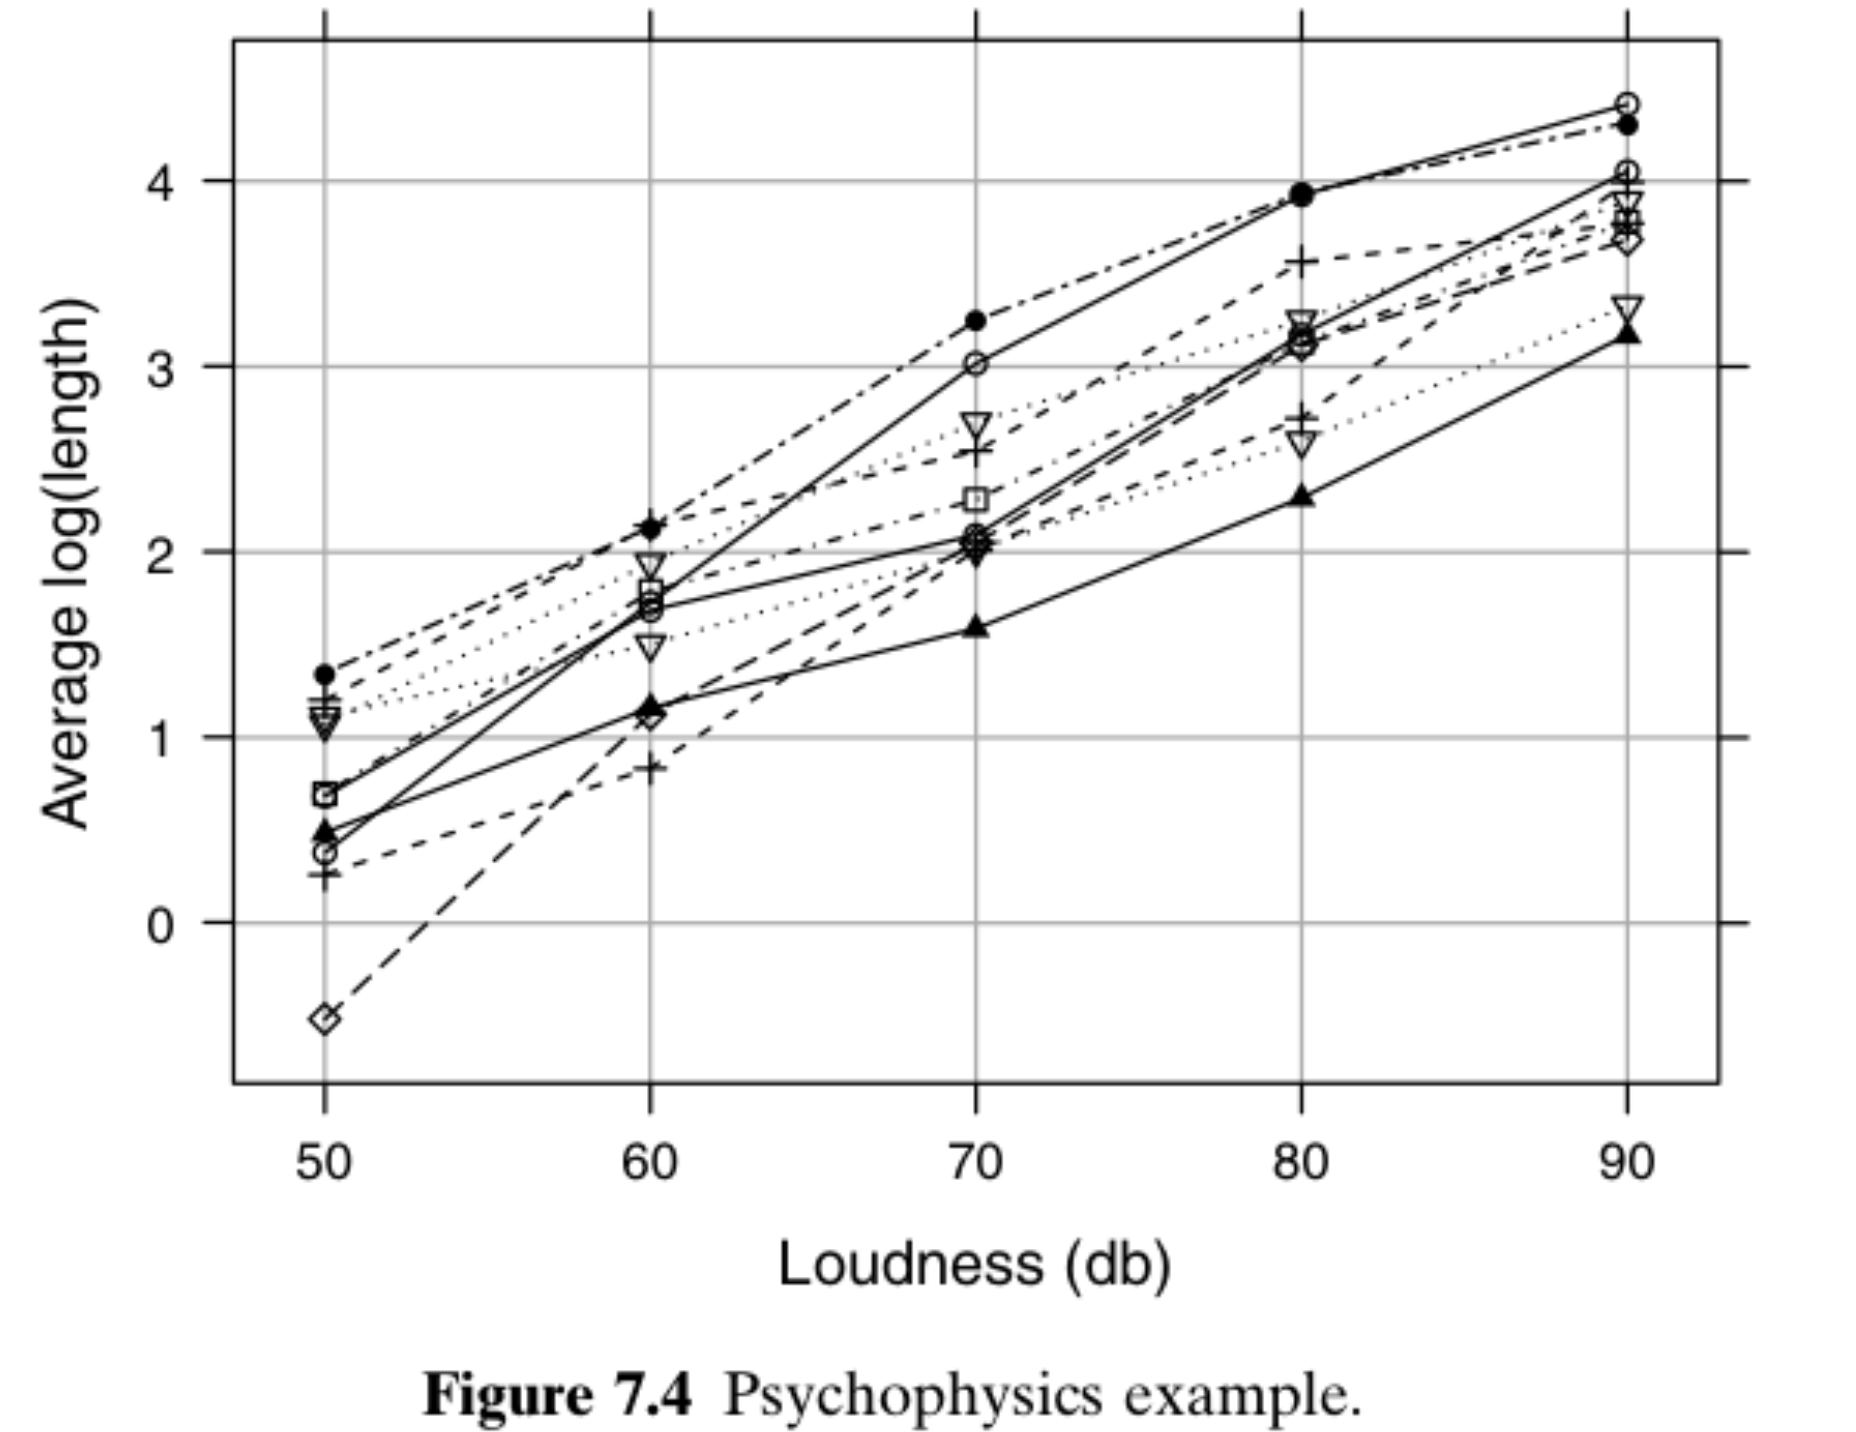
\includegraphics[width=1\textwidth]{fig12.png}
\end{figure} 
\begin{figure}[H]
    \centering
    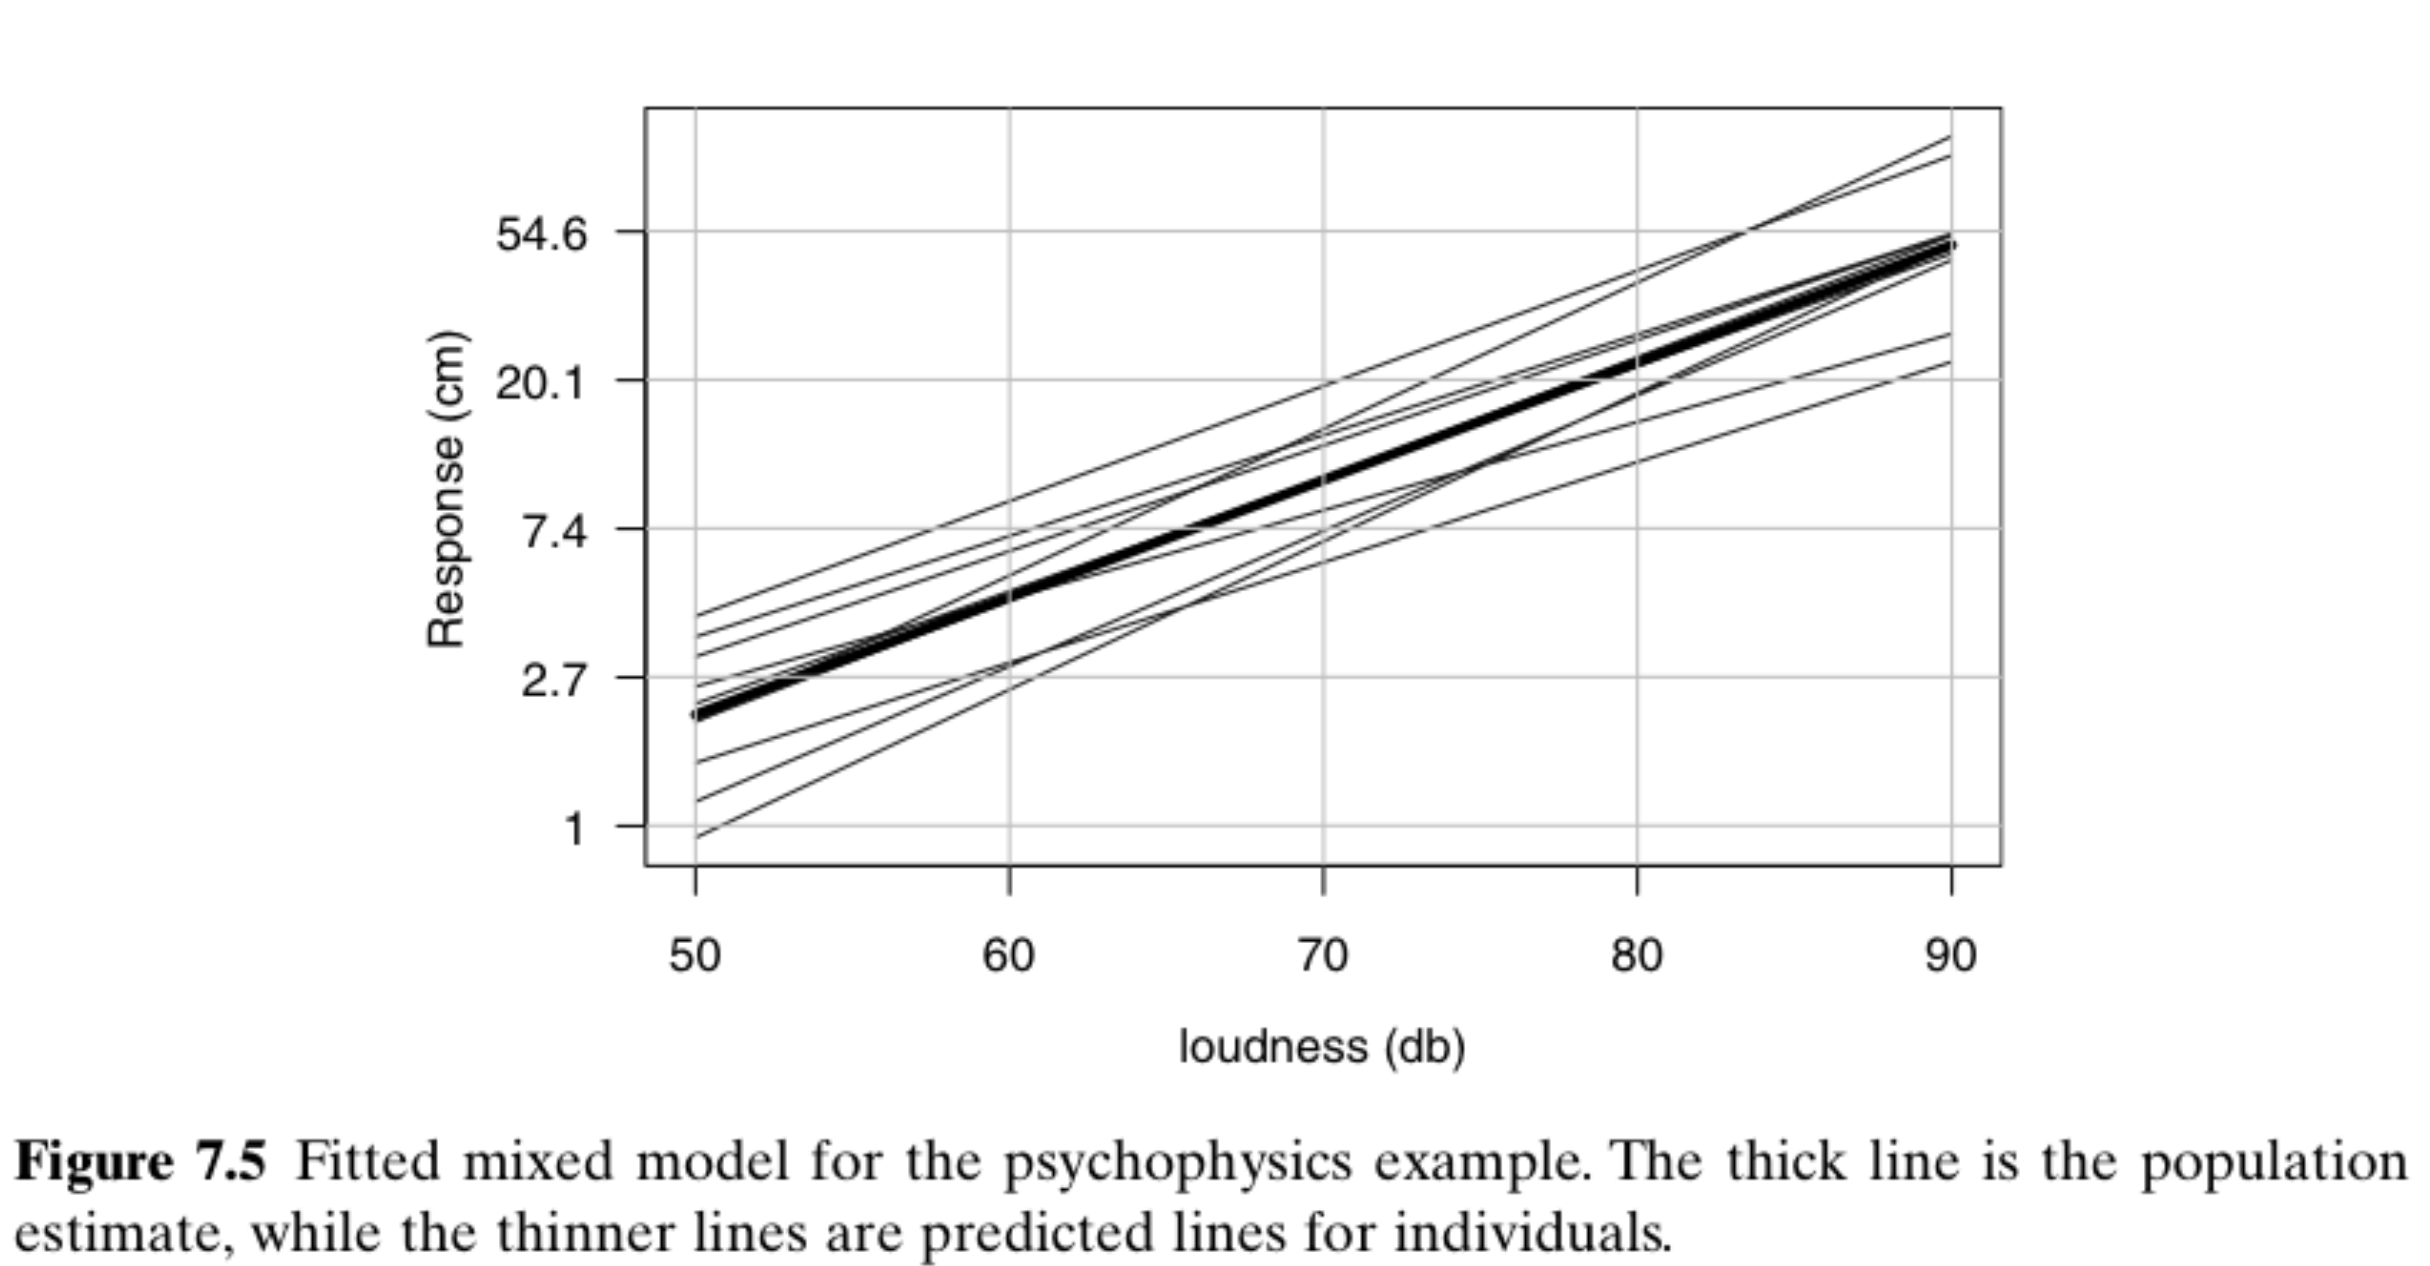
\includegraphics[width=1\textwidth]{fig13.png}
\end{figure} 
\section*{Variance Stabilizing Transformation}
\noindent
Suppose that the response is strictly positive, and the variance function before transformation is
\[
\text{Var}(Y | X = x) = \sigma^2 g(E(Y | X = x)),
\]
where \( g(E(Y | X = x)) \) is a function that is increasing with the value of its argument. For example, if the distribution of \( Y | X \) has a Poisson distribution, then \( g(E(Y | X = x)) = E(Y | X = x) \).\\
For distributions in which the mean and variance are functionally related, Scheffe (1959) provides a general theory for determining transformations that can stabilize variance. Table \# lists the common variance stabilizing transformations.
\begin{figure}[H]
    \centering
    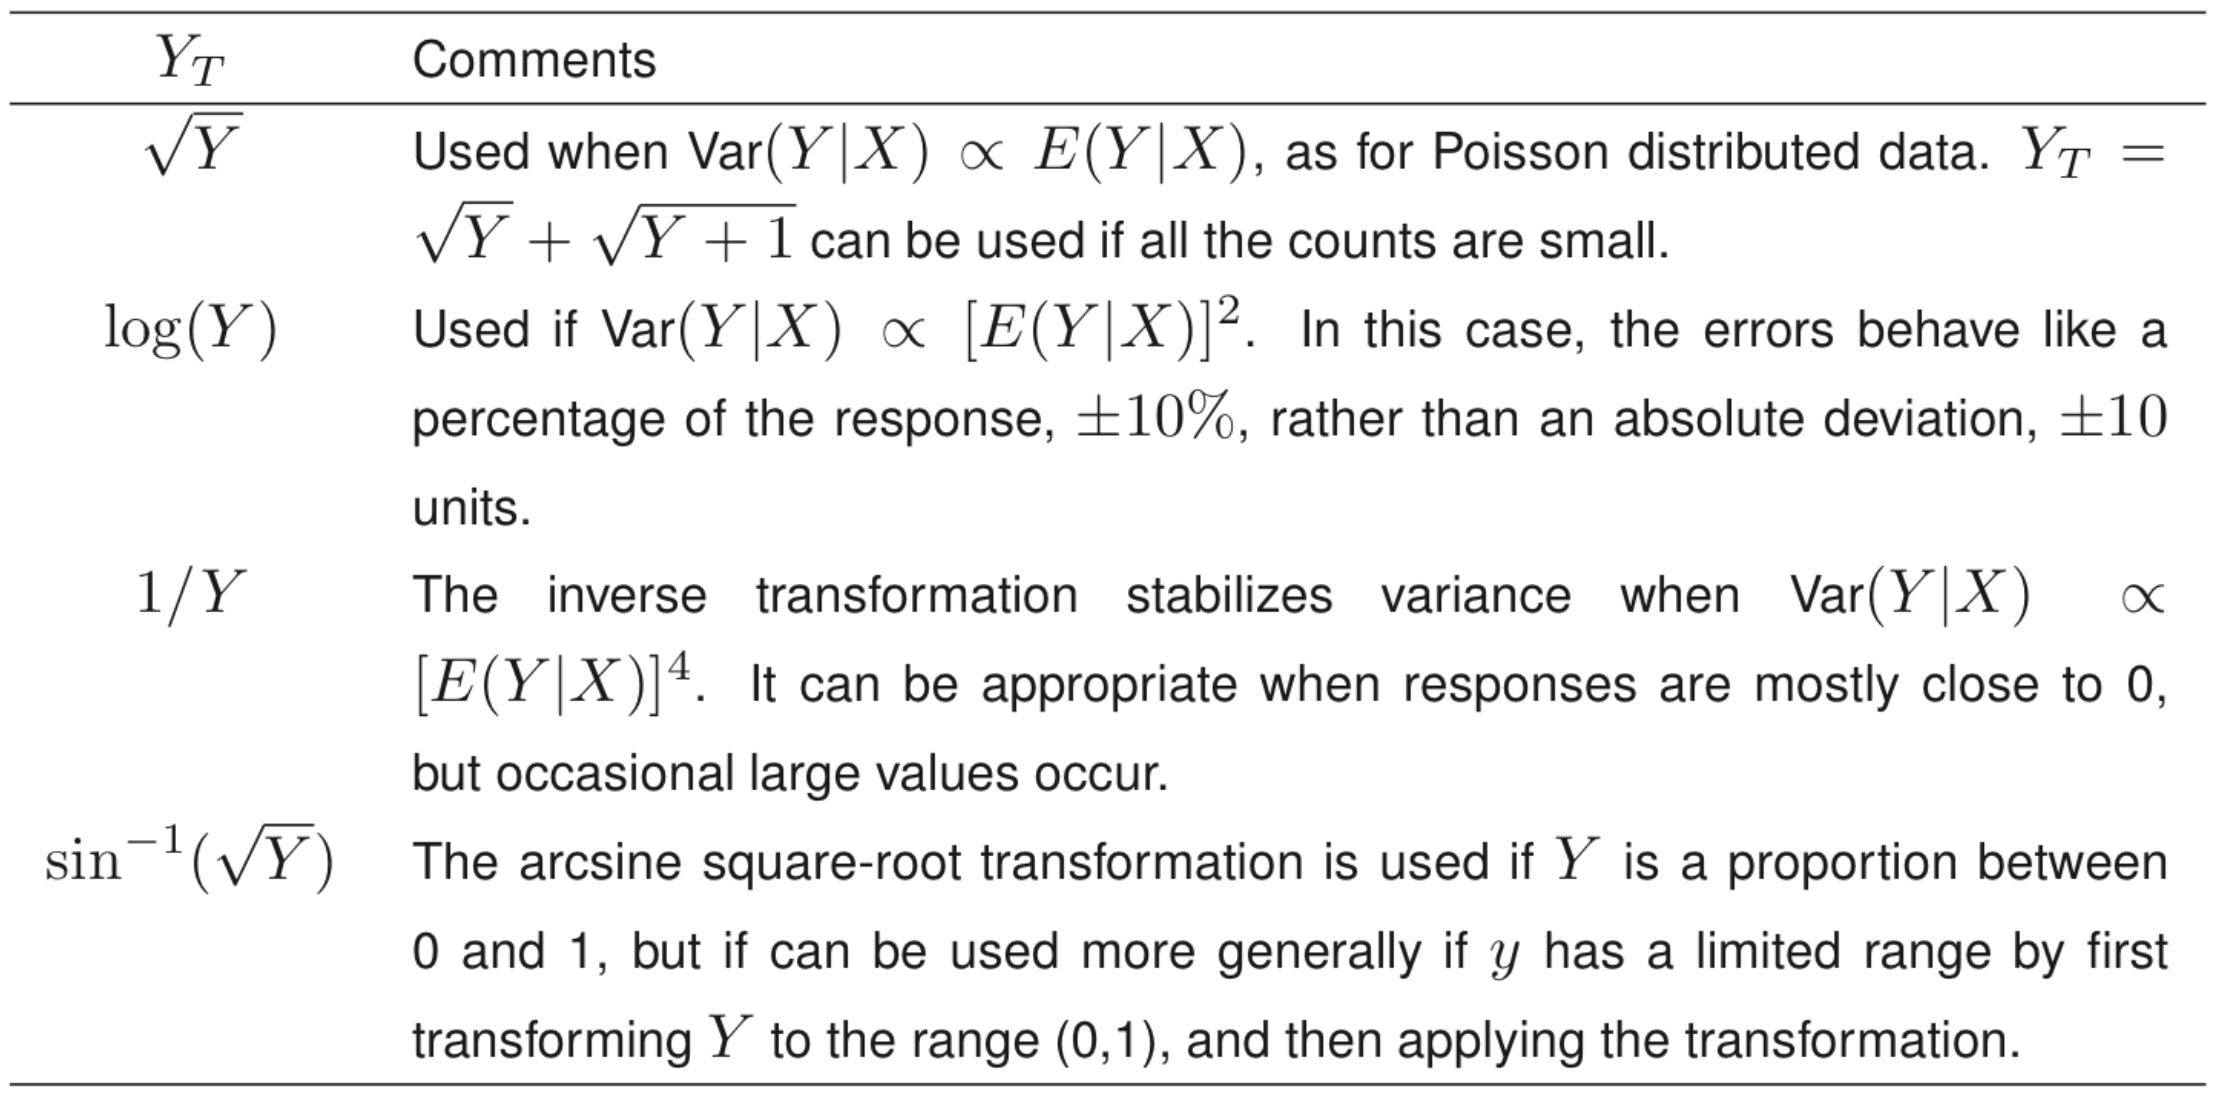
\includegraphics[width=1\textwidth]{fig14.png}
\end{figure} 
\section*{The Bootstrap}
\noindent
Suppose we have a sample \( y_1, \dots, y_n \) from a particular distribution \( G \), for example a standard normal distribution. What is a confidence interval for the population median?\\
We can obtain an approximate answer to this question by computer simulation, set up as follows.\\
1. Obtain a simulated random sample \( y_1^*, \dots, y_n^* \) from the known distribution \( G \).\\
2. Compute and save the median of the sample in step 1.\\
3. Repeat steps 1 and 2 a large number of times, say \( B \) times. The larger the value of \( B \), the more precise the ultimate answer.\\
4. If we take \( B = 999 \), a simple percentile-based \( 95\% \) confidence interval for the median is the interval between the sample 2.5 and 97.5 percentiles, respectively.\\
In most interesting problems, \( G \) is unknown and so this simulation is not available. Efron (1979) pointed out that the observed data can be used to estimate \( G \), and then we can sample from the estimate \( \hat{G} \). The algorithm becomes:\\
1. Obtain a random sample \( y_1^*, \ldots, y_n^* \) from \( \hat{G} \) by sampling with replacement from the observed values \( y_1, \ldots, y_n \). In particular, the \( i \)-th element of the sample \( y_i^* \) is equally likely to be any of the original \( y_1, \ldots, y_n \). Some of the \( y_i \) will appear several times in the random sample, while others will not appear at all.\\
2. Continue with steps 2-4 of the first algorithm. A test at the \( 5\% \) level concerning the population median can be rejected if the hypothesized value of the median does not fall in the confidence interval computed in step 4.\\
Efron called this method the \textit{bootstrap}.
\begin{figure}[H]
    \centering
    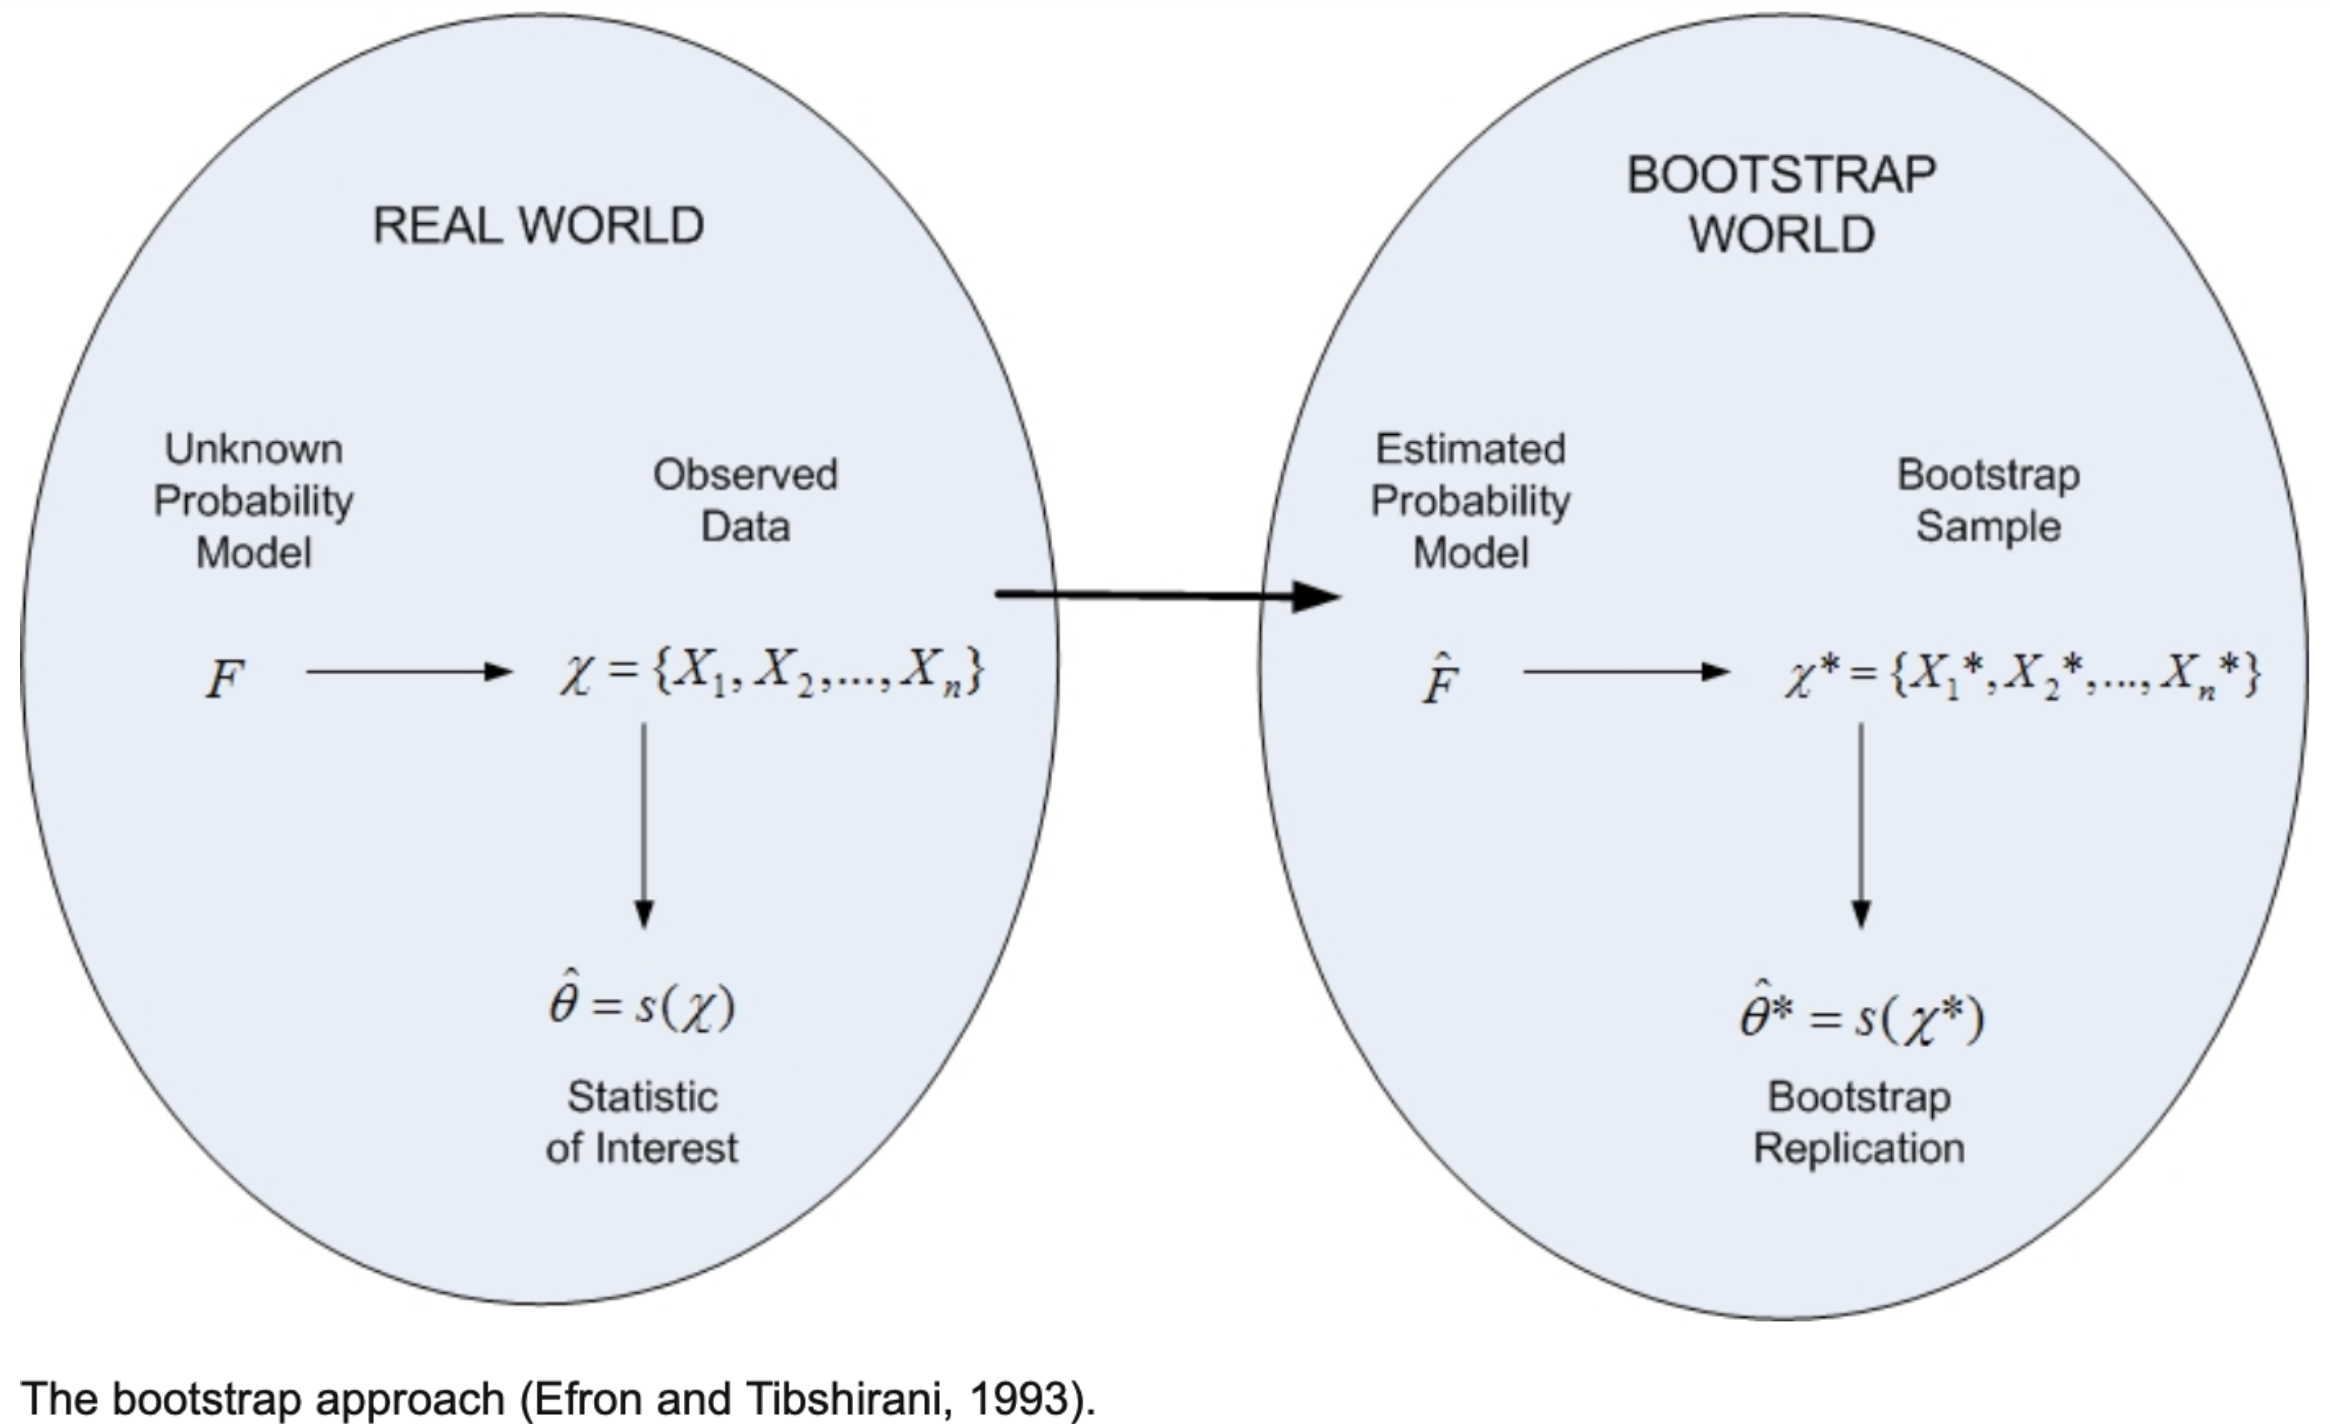
\includegraphics[width=1\textwidth]{fig15.png}
\end{figure} 
\section*{Regression Inference without Normality}
\noindent
For regression problems, when the sample size is small and the normality assumption does not hold, standard inference methods can be misleading, and in these cases a bootstrap can be used for inference.
\subsection*{Transactions Data}
Each branch makes transactions of two types, and for each of the branches we have recorded the number of transactions \( T_1 \) and \( T_2 \), as well as \textit{Time}, the total number of minutes of labor used by the branch in type 1 and type 2 transactions. The mean response function is
\[
E(\text{Time} | T_1, T_2) = \beta_0 + \beta_1 T_1 + \beta_2 T_2
\]
possibly with \( \beta_0 = 0 \) because zero transactions should imply zero time spent. The data are displayed in Figure 1. The marginal response plots in the last row appear to have reasonably linear mean functions; there appear to be a number of branches with no \( T_1 \) transactions but many \( T_2 \) transactions; and in the plot of \textit{Time} versus \( T_2 \), variability appears to increase from left to right.\\
\begin{figure}[H]
    \centering
    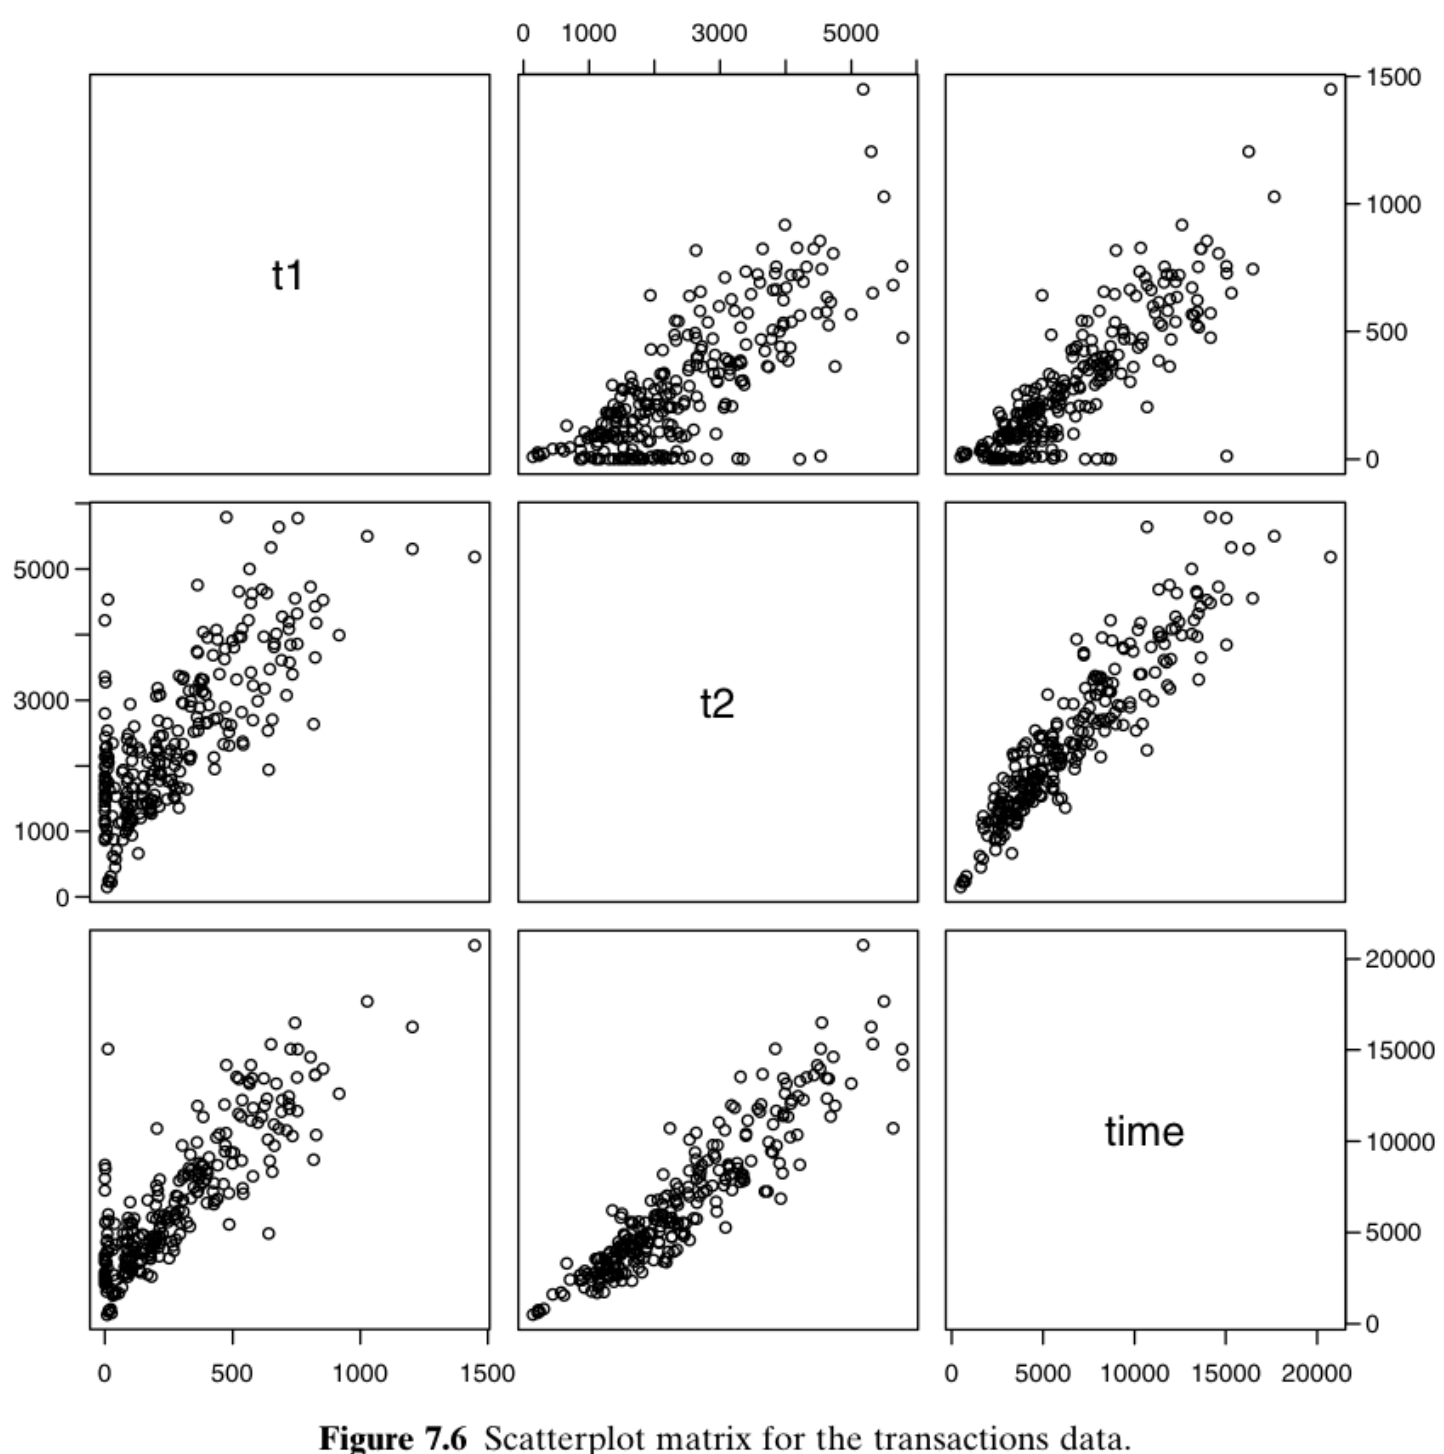
\includegraphics[width=1\textwidth]{fig16.png}
\end{figure} 
The errors in this problem probably have a skewed distribution. Occasional transactions take a very long time, but since transaction time is bounded below by zero, there cannot be any really extreme "quick" transactions. Inferences based on normal theory are therefore questionable.\\
A bootstrap is computed as follows.\\
1. Number the cases in the dataset from \( 1 \) to \( n \). Take a random sample (\textcolor{red}{from $\{(x_i, y_i) ; i = 1, \ldots, n\}
$}) with replacement of size \( n \) from these case numbers.\\
2. Create a dataset from the original data, but repeating each row in the dataset the number of times that row was selected in the random sample in step 1.\\
3. Repeat steps 1 and 2 a large number of times, say, \( B \) times.\\
4. Estimate a \( 95\% \) confidence interval for each of the estimates by the 2.5 and 97.5 percentiles of the sample of \( B \) bootstrap samples.\\
Table 6 summarizes the percentile bootstrap for the transaction data.\\
The \( 95\% \) bootstrap intervals are consistently wider than the corresponding normal intervals, indicating...
\begin{figure}[H]
    \centering
    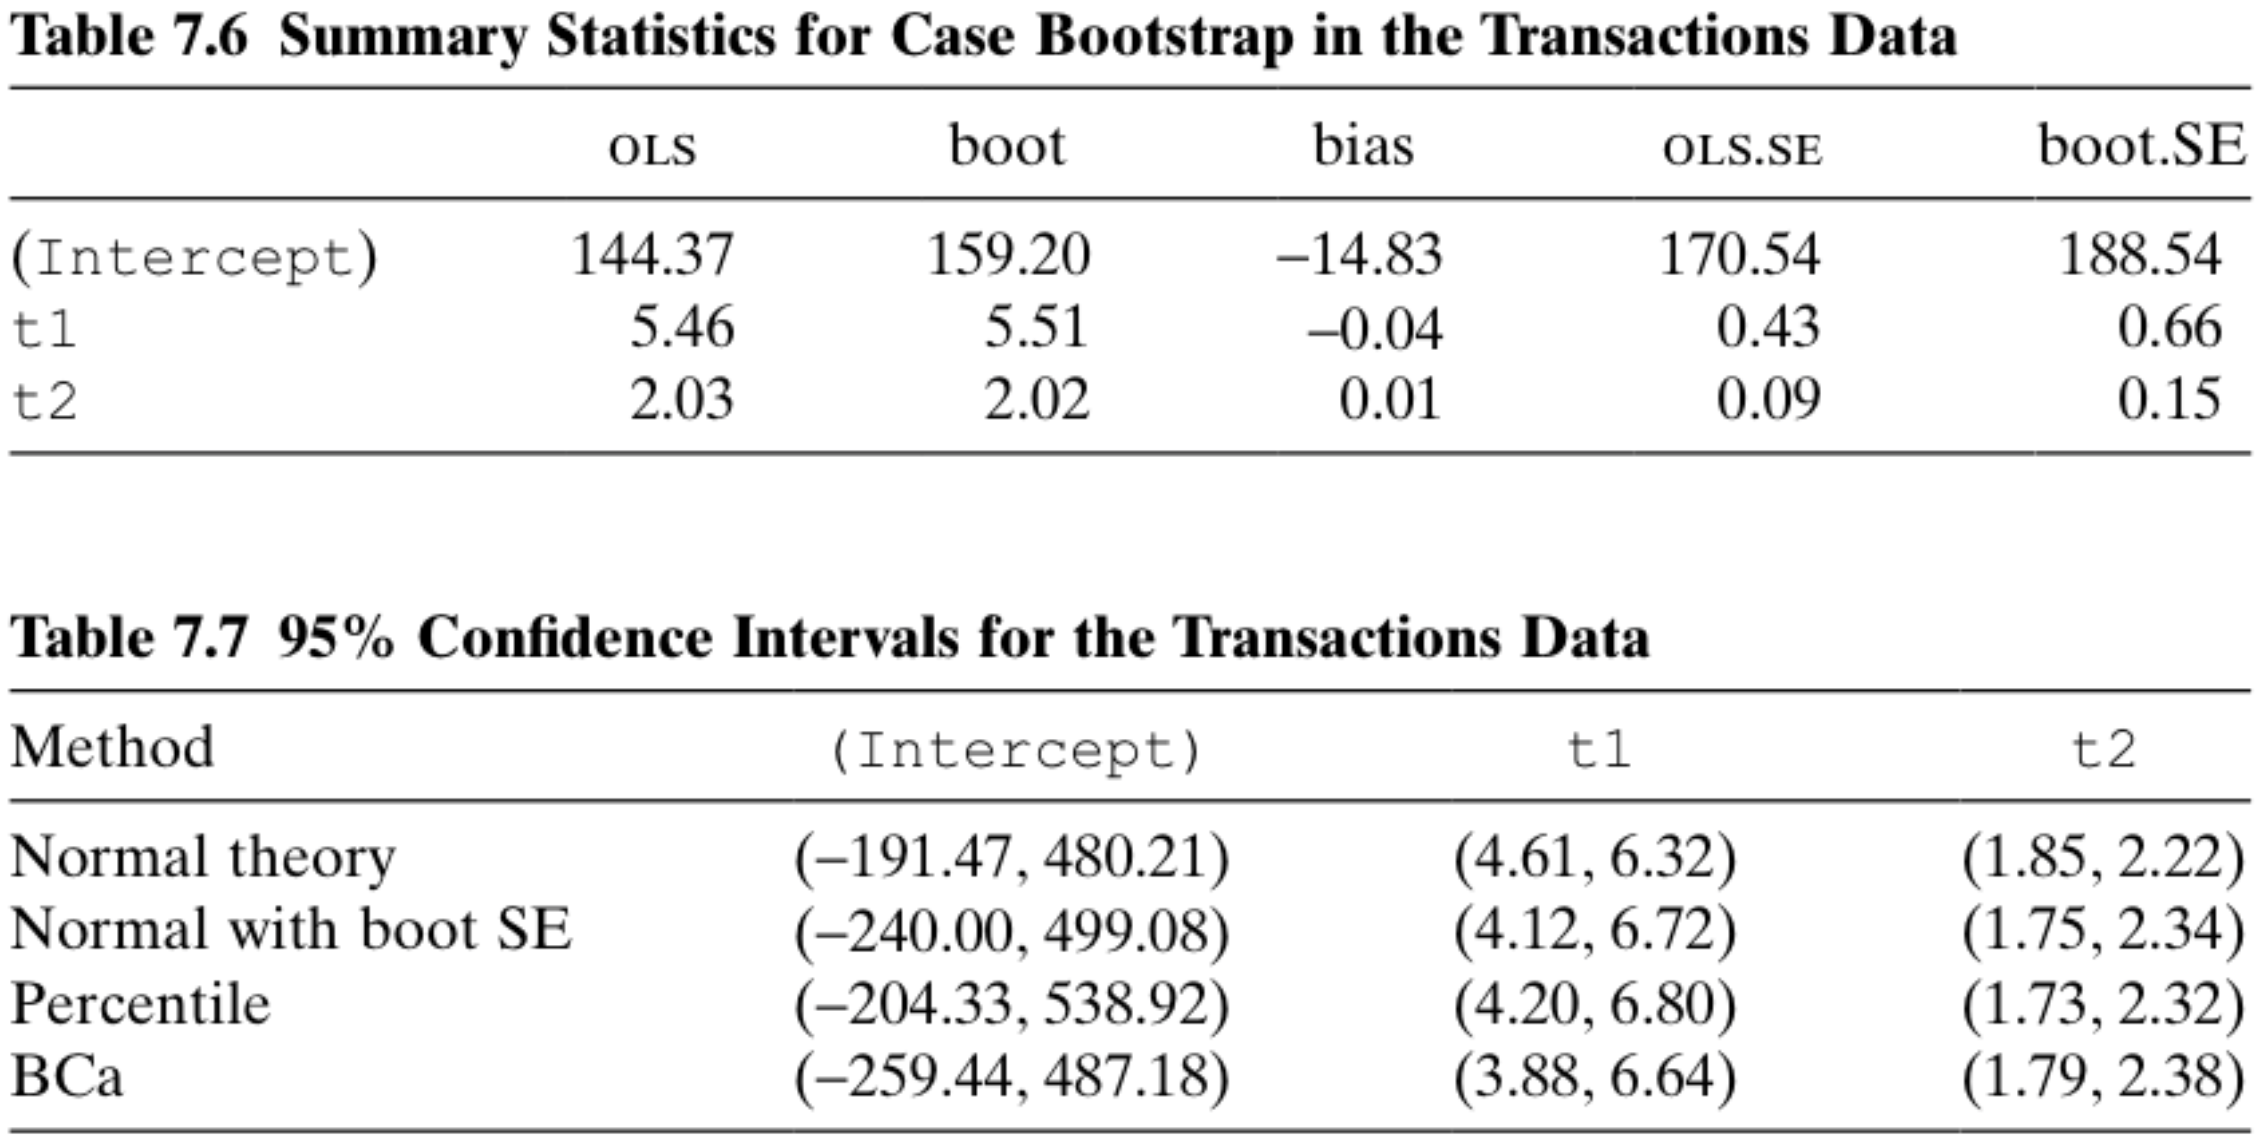
\includegraphics[width=1\textwidth]{fig17.png}
\end{figure} 
\subsection*{Residual Bootstrap}
1. Given data \((x_i, y_i), \, i = 1, \ldots, n\), fit the linear regression model \( E(Y|X = x) = \beta' x \) and compute the \textsc{ols} estimator \(\hat{\beta}\), and the residuals, \(\hat{e}_i = y_i - \hat{\beta}' x_i\).\\
2. Randomly sample from the residuals to get a new sample \((e_1^*, \ldots, e_n^*)\), where \(e_i^*\) is equally likely to be any of \((\hat{e}_1, \ldots, \hat{e}_n)\). A modified definition of residuals can be used that may slightly improve performance by correcting for unequal variances of the residuals; see Davison and Hinkley (1997, p. 262).\\
3. Create a bootstrap response with elements \(y_i^* = \hat{\beta}' x_i + e_i^*\). Compute the regression of the bootstrap response on \(X\), and get the coefficient estimates or other summary statistic of interest.\\
4. Repeat steps 2 and 3 \(B\) times. Confidence intervals are obtained as with the case bootstrap.








\end{document}